\documentclass[10pt, twoside]{article} % Rozmiar czcionki 10, marginesy lustrzane (1) i justowanie do obydwu marginesów

% Compiler: LuaLaTex

% do zbiorow
\usepackage{amsmath}
\usepackage{amssymb}
\usepackage{bm}


% figure, subfigure
\usepackage{caption}
\usepackage{subcaption}
\usepackage{graphicx}

\numberwithin{equation}{subsection}
\usepackage{fontspec} % Wymagane do ustawienia czcionki
\setmainfont{Arial} % Czcionka (rodzaj)

\usepackage[a4paper,
top=2.5cm, 
bottom=2.5cm, 
inner=2.5cm, 
outer=3.5cm, 
twoside]{geometry} % Marginesy lustrzane (2)

\usepackage{setspace} % Wymagane do ustawienia interlinii
\onehalfspacing % Interlinia 1.5 wiersza

\setlength{\parindent}{1.25cm} % Wcięcie w akapitach 1.25 cm
\usepackage{indentfirst} % Wcięcie (w akapitach) również na początku (sub)sekcji

% Wymagane do ustawienia numeracji stron - - - - - - - - - - - - - - - - - -
\usepackage{fancyhdr} % Niezbędny pakiet
\pagestyle{fancy} % Wykorzystanie fancyhdr
\fancyfoot{} % Wyczyszczenie ustawień nagłówka 
\fancyhead{} % Wyczyszczenie ustawień stópki
\renewcommand{\headrulewidth}{0pt} % Usunięcie linii z nagłówka
\renewcommand{\footrulewidth}{0pt} % Usunięcie linii ze stópki
\setcounter{page}{1} % Numerowanie od 3, a nie 1
\fancyfoot[C]{\fontsize{9pt}{11pt}\selectfont \thepage} % Czcionka Arial o rozmiarze 9 z wyśrodkowaniem
% Wymagane do ustawienia numeracji stron - - - - - - - - - - - - - - - - - -

\AddToHook{cmd/section/before}{\clearpage} % Każda sekcja na nowej stronie

% Wymagane do sformatowania tytułów rozdziałów - - - - - - - - - - - - - - - - - -
\usepackage{titlesec} % Niezbędny pakiet
\titlespacing*{\section} % Definicja odstępów dla sekcji
{0pt} % Wcięcie od lewej
{12pt} % Miejsce nad tytułem sekcji
{6pt} % Miejsce poniżej tytułu sekcji
\titlespacing*{\subsection}{0pt}{12pt}{6pt} % Definicja odstępów dla subsekcji
\titlespacing*{\subsubsection}{0pt}{12pt}{6pt} % Definicja odstępów dla subsubsekcji
\titleformat{\section}
{\normalfont\fontsize{12pt}{14pt}\selectfont\bfseries\MakeUppercase} % Pogrubienie + wielkie litery + rozmiar 12pt
{\thesection.}{1em}{} % Numeracja z kropką, odstęp 1em
\titleformat{\subsection}{\normalfont\fontsize{10pt}{12pt}\selectfont\bfseries\itshape}{\thesubsection.}{1em}{} % Pogrubienie, rozmiar 10pt i pochylenie
\titleformat{\subsubsection}{\normalfont\fontsize{10pt}{12pt}\selectfont\itshape}{\thesubsubsection.}{1em}{} % Pochylenie i rozmiar 10pt
% Wymagane do sformatowania tytułów rozdziałów - - - - - - - - - - - - - - - - - -

\titlelabel{\thetitle.\quad} % Kropka po numerze tytułu (sub)sekcji

% Wymagane do sformatowania spisu treści - - - - - - - - - - - - - - - - - -
\usepackage{tocloft} % Niezbędny pakiet
\renewcommand{\cftsecleader}{\cftdotfill{\cftdotsep}} % [numer sekcji] [kropka] [nazwa] *[kropki]* [numer strony]
% [numer sekcji] *[kropka]* [nazwa] [kropki] [numer strony] - - -
\renewcommand{\cftsecaftersnum}{.}
\renewcommand{\cftsubsecaftersnum}{.}
\renewcommand{\cftsubsubsecaftersnum}{.}
% [numer sekcji] *[kropka]* [nazwa] [kropki] [numer strony] - - -
% Górny odstęp 0 pkt - - -
\renewcommand{\cftbeforesecskip}{0pt}
\renewcommand{\cftbeforesubsecskip}{0pt}
\renewcommand{\cftbeforesubsubsecskip}{0pt}
% Górny odstęp 0 pkt - - -
% Dolny odstęp 6 pkt - - -
\renewcommand{\cftsecafterpnum}{\vskip6pt}
\renewcommand{\cftsubsecafterpnum}{\vskip6pt}
\renewcommand{\cftsubsubsecafterpnum}{\vskip6pt}
% Dolny odstęp 6 pkt - - -
% Automatycznie duże litery sekcji?
% Wymagane do sformatowania spisu treści - - - - - - - - - - - - - - - - - -

\usepackage{csquotes} % Potrzebny do BiblaTex
\usepackage[
backend=biber,
style=numeric-comp, % [numer] + pojawią się zakresy, np. [1-2]
sorting=none % Sortowanie według kolejności występowania
]{biblatex} % Ustawienia bibliografii
\addbibresource{full_bibliography.bib} % Załączenie bibliografii

\usepackage{etoolbox} % Potrzebny do modyfikacji akapitów bibliografii
\AtBeginBibliography{\setlength{\parskip}{6pt} \setlength{\parindent}{0pt}} % Dolny odstęp 6 pt, górny odstęp 0 pt
\renewcommand*{\finentrypunct}{\par} % Zapewnia, że po każdym wpisie bibliograficznym jest akapit

\usepackage{graphicx} % Wymagane do wstawiania obrazów

% Formatowanie podpisu obrazków - - - - - - - - - - - - - - - - - -
\usepackage[figurename=Fig.]{caption} % Niezbędny pakiet
\usepackage{chngcntr} % Wymagane do zmiany numeracji
\counterwithin{figure}{section} % Numeracja obrazków zależna od sekcji (rozdziału)
\renewcommand{\thefigure}{\thesection.\arabic{figure}} % Format numeracji obrazków
\captionsetup[figure]{
	font=small,                % Rozmiar czcionki (około 9pt)
	labelformat=simple,        % Format etykiety (np. "Rysunek 1")
	labelsep=period,           % Separator między etykietą a opisem
	justification=centering,   % Wyśrodkowanie podpisu
	% skip=12pt,               % Odstęp między obrazkiem a podpisem
	textfont=normalfont,       % Czcionka normalna, bez kursywy
	belowskip=-6pt,            % Dolny odstęp akapitu podpisu
	% aboveskip=6pt,           % Górny odstęp akapitu podpisu
	% parskip=0pt,             % Odstęp między akapitami podpisu
	format=plain,              % Formatowanie podpisu, brak kropki na końcu
} % Formatowanie podpisu pod obrazkami
% Formatowanie podpisu obrazków - - - - - - - - - - - - - - - - - -

% Formatowanie podpisu tabel - - - - - - - - - - - - - - - - - -
\usepackage[table,xcdraw]{xcolor} % Niezbędny pakiet
\counterwithin{table}{section} % Numeracja tabel zależna od sekcji (rozdziału)
\renewcommand{\thetable}{\thesection.\arabic{table}} % Format numeracji tabel
\captionsetup[table]{
	font=small,                % Rozmiar czcionki (około 9pt)
	labelformat=simple,        % Format etykiety (np. "Tab. 1")
	labelsep=period,           % Separator między etykietą a opisem
	justification=centering,   % Wyśrodkowanie podpisu
	% skip=12pt,               % Odstęp między tabelą a podpisem
	textfont=normalfont,       % Czcionka normalna, bez kursywy
	belowskip=-6pt,            % Dolny odstęp akapitu podpisu
	% aboveskip=6pt,           % Górny odstęp akapitu podpisu
	% parskip=0pt,             % Odstęp między akapitami podpisu
	format=plain,              % Formatowanie podpisu, brak kropki na końcu
} % Formatowanie podpisu pod tabelami
% Formatowanie podpisu tabel - - - - - - - - - - - - - - - - - -

\usepackage{enumitem} % Wymagane do zmiany odległości pomiędzy wierszami w listach

\usepackage{hyperref} % Podświetlanie URL, źródeł i zakładek z opcją przeniesienia na kliknięcie (widoczne tylko przed eksportem)

\usepackage{lscape} % Wymagane do zmiany orientacji tabeli
\usepackage{longtable} % Wymagane do tabelii na wielu stronach

% Wymagane do listingów - - - - - - - - - - - - - - - - - - - - - - - - - - - - - -
\usepackage{listings} % Wymagany pakiet
\usepackage{xcolor} % Potrzebne do poprawnego wyświetlania listingów
% Definicja kolorów
\definecolor{codeblue}{rgb}{0.26, 0.48, 0.77}
\definecolor{codegreen}{rgb}{0.13, 0.54, 0.13}
\definecolor{codegray}{rgb}{0.5, 0.5, 0.5}
\definecolor{codepurple}{rgb}{0.58, 0, 0.82}
\definecolor{backcolor}{rgb}{0.95, 0.95, 0.92}
% Konfiguracja języka TypeScript
\lstdefinelanguage{Python}{
	keywords={def, class, return, if, elif, else, for, while, break, continue, pass, import, from, as, lambda, with, try, except, finally, raise, assert, yield, global, nonlocal, async, await},
	keywordstyle=\color{codeblue}\bfseries, % Keywords in blue
	ndkeywords={True, False, None},
	ndkeywordstyle=\color{codepurple}, % Special values in purple
	identifierstyle=\color{black}, % Variable names in black
	sensitive=true, % Case-sensitive
	comment=[l]{\#}, % Single-line comments
	morecomment=[s]{'''}{'''}, % Multi-line comments with triple single quotes
	morecomment=[s]{"""}{"""}, % Multi-line comments with triple double quotes
	commentstyle=\color{codegreen}\ttfamily, % Comments in green
	stringstyle=\color{orange}\ttfamily, % Strings in orange
	morestring=[b]', % Single and double quotes
	morestring=[b]"
}
% Ogólne ustawienia dla listingów
\lstset{
	language=Python,               % Język programowania
	backgroundcolor=\color{backcolor}, % Tło dla kodu
	basicstyle=\ttfamily\small,        % Podstawowy styl czcionki
	keywordstyle=\color{codeblue}\bfseries, % Kolorowanie słów kluczowych
	ndkeywordstyle=\color{codepurple}, % Kolorowanie specjalnych wartości
	commentstyle=\color{codegreen}\ttfamily, % Styl komentarzy
	stringstyle=\color{orange}\ttfamily,     % Styl łańcuchów znaków
	numbers=left,                     % Numerowanie linii po lewej stronie
	numberstyle=\tiny\color{codegray},% Styl numerów linii
	stepnumber=1,                     % Co ile numerować linie
	frame=single,                     % Ramka wokół kodu
	rulecolor=\color{codegray},       % Kolor ramki
	breaklines=true,                  % Automatyczne łamanie długich linii
	tabsize=2,                        % Rozmiar tabulatora
	showspaces=false,                 % Nie pokazuj spacji
	showstringspaces=false            % Nie pokazuj spacji w łańcuchach znaków
}
% Wymagane do listingów - - - - - - - - - - - - - - - - - - - - - - - - - - - - - -

\usepackage{pdfpages} % Wymagane do załączenia pliku PDF

\begin{document}
	
	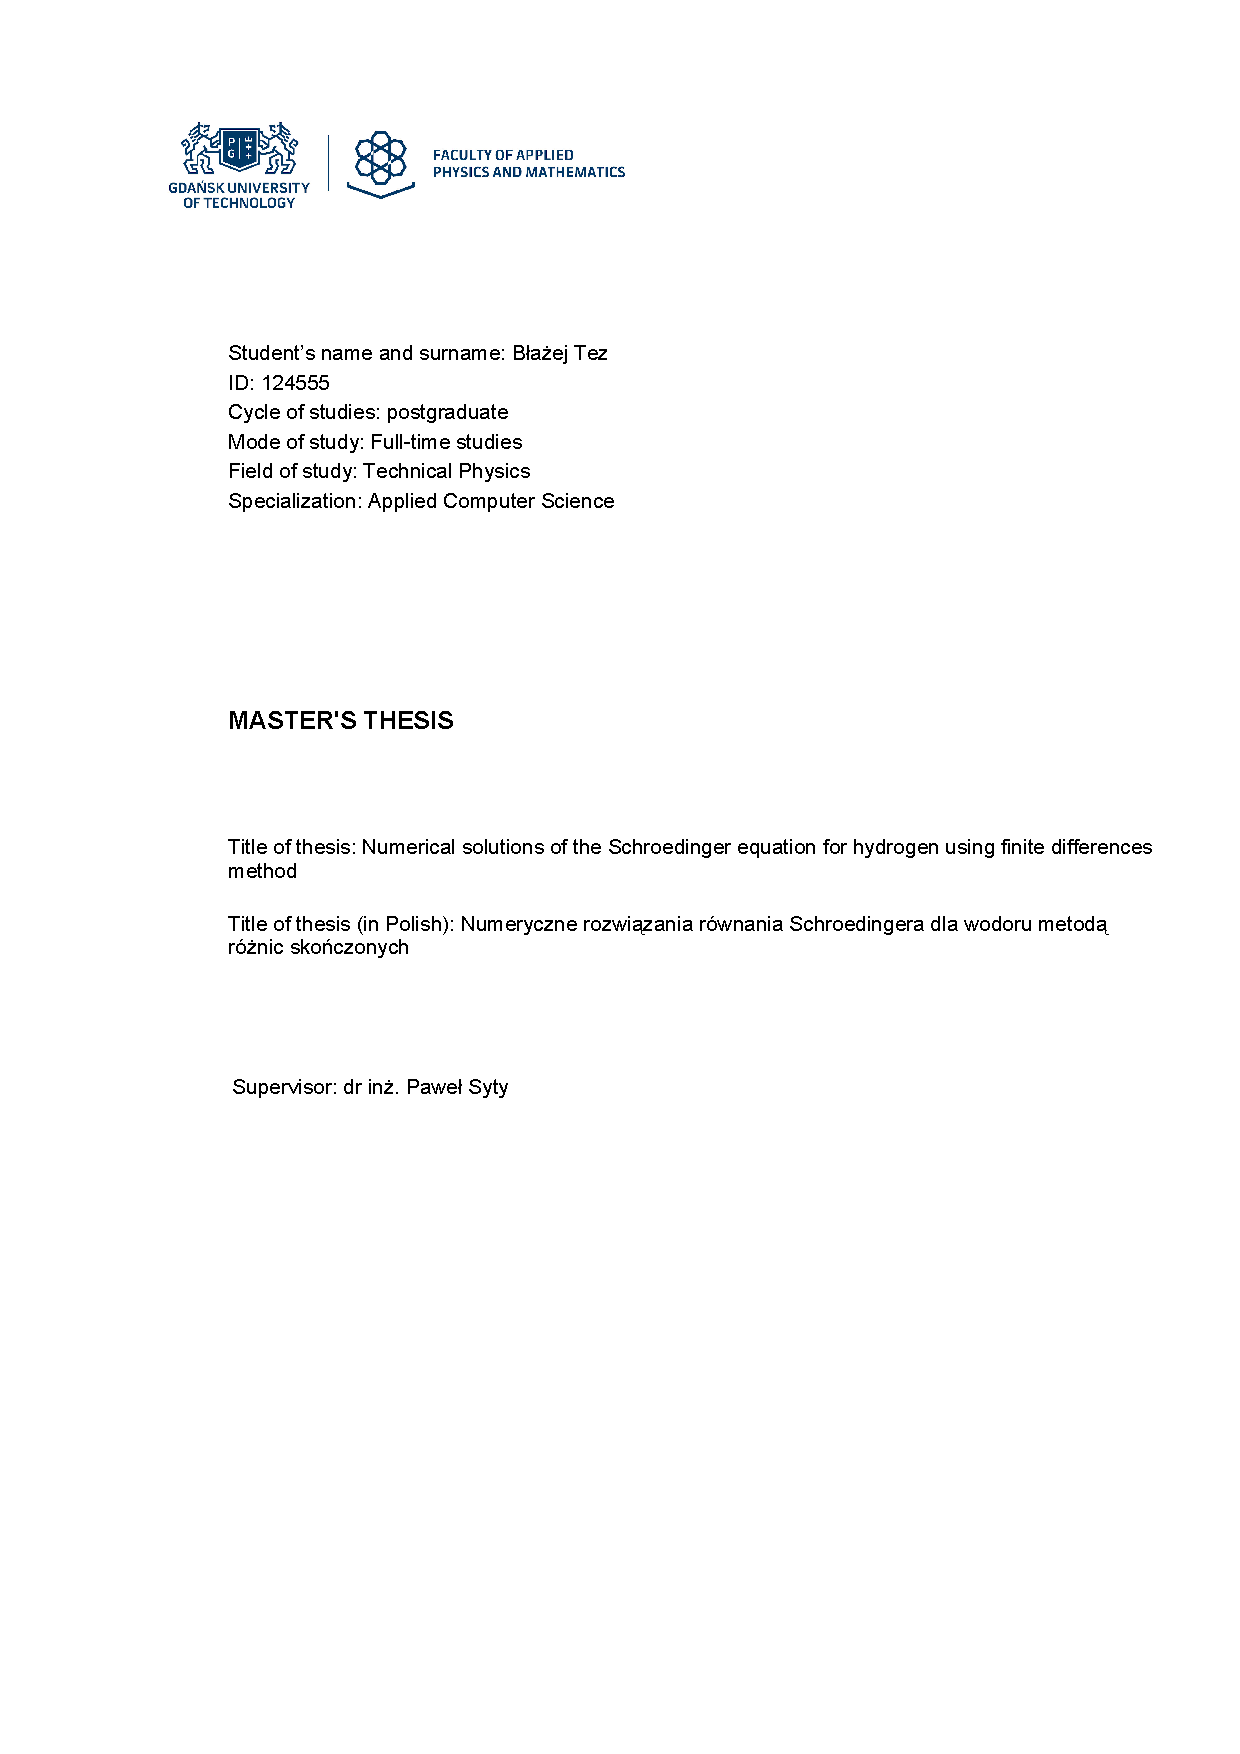
\includepdf[pages=-, pagecommand={\thispagestyle{empty}}]{title_page.pdf}
	
%	\includepdf[pages=-, pagecommand={\thispagestyle{empty}}]{Oswiadczenie.pdf}
	
	\noindent
\begingroup
\fontsize{12pt}{1.5pt}\selectfont
\textbf{STRESZCZENIE}
\endgroup

\vspace{3mm}

Od momentu pojawienia się architektury Compute Unified Device Architecture (CUDA), badacze zyskali możliwość rozwiązywania w efektywniejszy sposób skomplikowanych obliczeniowo problemów, osiągając szybsze wyniki i większą dokładność numeryczną. Niniejszy projekt wpisuje się w ten trend, zawierając nową metodę obliczania stanu podstawowego i stanów wzbudzonych atomu wodoru z wykorzystaniem metody różnic skończonych. Implementację nowej metody i testy wykonano na konsumenckiej karcie graficznej o najwyższych możliwościach obliczeniowych w momencie publikacji, a mianowicie Nvidia RTX 4090.

Większość projektu została opracowana w języku Python z wykorzystaniem biblioteki CuPy, z wyłączeniem fragmentów zaimplementowanych wprost w CUDA C.

Ponadto w ramach tej pracy porównano algorytmy numeryczne służące do rozwiązywania problemu własnego równania Schr{\"o}dingera w celu optymalizacji minimalizacji ilorazu Rayleigha. Uzyskane funkcje falowe zostały zwizualizowane z wykorzystaniem mayavi - modułu z języka Python, a wyniki porównano z reprezentacjami graficznymi analitycznie wyprowadzonych funkcji falowych.

\textbf{Słowa kluczowe:}: metoda różnic skończonych, równanie Schrödingera, atom wodoru.

\textbf{Dziedzina i dyscyplina naukowa zgodnie z wymaganiami OECD:}
nauki komputerowe i informatyczne, informatyka
	\newpage
	\noindent
\begingroup
\fontsize{12pt}{1.5pt}\selectfont
\textbf{ABSTRACT}
\endgroup

\vspace{3mm}

Ever since the introduction of the Compute Unified Device Architecture (CUDA), researchers have gained the capability to solve computationally challenging problems more efficiently, leading to faster results and greater numerical accuracy. This thesis contributes to this trend by introducing a novel approach for calculating hydrogen energy through Schr{\"o}dinger equation with finite difference method. By avoiding the need to explicitly store Hamiltonian operator matrix, the approach removes the $O(x^6)$ space complexity. The new solution was implemented and tested on the best high-performance customer graphics card available in 2024, the Nvidia RTX 4090.

Most of the project was developed in Python using the CuPy library, while some fragments were implemented in CUDA C. This work includes the implementation of several numerical algorithms for solving the Schrödinger equation eigenproblem through minimization of Rayleigh's quotient, as well as using existing LOBPCG algorithm implementation. The resulting wavefunctions were visualized using the mayavi Python module, with comparisons made to analytical solutions of hydrogen atom wavefunctions.

\textbf{Keywords:} finite difference method, Schrödinger equation, hydrogen atom.

\textbf{Field and science of technology in accordance with OECD requirements:}
physical science, computer and information sciences, computer sciences

	
	\newpage
	\begin{singlespace} % Interlinia 1
		\tableofcontents
	\end{singlespace}
	\thispagestyle{fancy} % Potrzebne, żeby dla strony tytułowej zadziałało formatowanie dla numeracji stron (rozmiar i rodzaj czcionki)
	
	\newpage
	\addcontentsline{toc}{section}{List of Key Symbols and Abbreviations}
\noindent
\begingroup
    \fontsize{12pt}{1.5pt}\selectfont
    \textbf{List of Key Symbols and Abbreviations}
\endgroup

\vspace{3mm}

\noindent GPU -- Graphics Processing Unit\newline
CPU -- Central Processing Unit\newline
CUDA -- Compute Unified Device Architecture\newline
STEM - Science, Technology, Engineering, Mathematics\newline
LOBPCG -- Locally Optimal Block Preconditioned Conjugate Gradient\newline
Adam -- Adaptive Moment Estimation\newline
FDM -- Finite Difference Method\newline
CDS -- Central Difference Scheme\newline
HOC -- High-Order Compact (finite difference scheme)\newline
SVD -- Stochastic Gradient Descent \newline
RMSP -- Root Mean Square Propagation\newline
HPC -- High Performance Computing\newline
FLOPS -- Floating-Point Operations Per Second\newline
F2P -- FLOP To Byte Ratio\newline
DRAM -- Dynamic Random-Access Memory\newline
VRAM -- Video Dynamic Random-Access Memory
	
	\section{Introduction}

\subsection{Background}
% ok, czyli mówię, że inaczej się liczy niż kiedyś
% czy chcę o Kołosie jak przyjechał z działającym programem do USA...?

The landscape of scientific computation has substantially evolved since Schrödinger introduced his famous equation. Modern scientists possess tools that are far more advanced than pen and paper, enabling them to solve complex mathematical problems with accuracy and speed greater than ever. Numerical methods, once laborious and prone to human error due to iterative processes, have become indispensable in many STEM disciplines.

Graphics Processing Units (GPUs) have proven to be highly effective, powerful, high-throughput computing units. While Central Processing Units (CPUs) have been optimized for low-latency tasks, addressing more minor problems quickly, the scientific and high-performance computing communities have demanded greater throughput for large-scale data processing. This demand led to the Compute Unified Device Architecture (CUDA) development in 2006, which allowed GPUs to be harnessed as general-purpose computing devices.

GPUs' parallel processing capabilities align perfectly with numerical methods like FDM, which often involves computations on large grids. By distributing these calculations across thousands of cores, GPUs significantly reduce computation time, making them ideal for large-scale simulations in quantum mechanics.

According to Nvidia, the number of CUDA-enabled devices used worldwide surpassed 500 million -- and that information has yet to be updated in the last three years, which was the time of the company's exponential growth in sales. The wide range of applications included bioinformatics, computational chemistry, fluid dynamics, structural mechanics, data science, numerical analytics, and many others.\cite{cuda} 	

\subsection{Problem statement}

This study aims to develop a new efficient method for solving the Schrödinger Equation using the Finite Difference Method (FDM) on a GPU while reducing memory complexity. The traditional approach of directly representing the Hamiltonian matrix results in memory requirements that grow as $O(x\textsuperscript{6})$, making large-scale quantum simulations challenging to handle on modern GPUs. This research aims to express the Laplacian part of Hamiltonian indirectly through the FDM, significantly reducing the space complexity to $O(x\textsuperscript{3})$, where x represents the edge length of the Cartesian grid.
%% poniższy akapit do przedyskutowania
In addition to reducing memory complexity, this work will employ numerical methods to solve the eigenvalue problem in a search for the most suitable one. These methods include minimizing Rayleigh's quotient, both with and without orthogonal vector constraints, using a variety of algorithms, including gradient descent, perturbed gradient descent, LOBPCG, and ADAM.

Finally, the proposed method has to be validated. For that purpose, this study aims to calculate the hydrogen atom's energies and their respective eigenstates. The hydrogen atom has well-known analytical solutions, which is favorable for serving as a benchmark for evaluating the new method's accuracy. By comparing the results to analytical solutions, this work will demonstrate the validity of the approach in solving quantum mechanical problems.

\subsection{Significance of the study}

This study addresses a critical challenge in computational quantum mechanics: how to efficiently and accurately solve the Schrödinger equation. The method proposed in this work significantly reduces the memory complexity of solving the Schrödinger equation using the FDM. By lowering the complexity from $O(x\textsuperscript{6})$ to $O(x\textsuperscript{3})$, this study may lead to more extensive and intricate quantum systems to be simulated on GPUs. This is particularly relevant for the design of new materials, drug discovery, and quantum technologies, where accurate quantum models enable better predictions of drug properties, guide experimental work, and foster innovation.

\subsection{Thesis Structure}

The subsequent chapters of this thesis focus on the following aspects of the work:
\begin{itemize}[itemsep=0\baselineskip, topsep=1.5pt, parsep=1.5pt] 
	\item Chapter 2 describes selected existing methods for solving the Schrödinger equation.
	\item Chapter 3 outlines this study's theoretical framework and software tools. The chapter also highlights the integration of Python, CuPy, and CUDA to optimize numerical computations on GPUs.
	\item Chapter 4 presents the results delivered by the new method, including a comparative analysis of different tools and approaches.
	\item Chapter 5 offers conclusions based on the obtained results and proposes directions for future research.  
	\item The appendix contains detailed proofs derived manually during the development of this thesis. These proofs include mathematical derivations of Laplace operator stencils and optimization steps for numerical solvers.
\end{itemize}


	
	\section{EXISTING WAYS TO SOLVE SCHRÖDINGER EQUATION FOR HYDROGEN ATOM}

\subsection{Analytical Solution}

The potential of exact solutions is significantly constrained by the rapidly escalating complexity introduced by each additional body in the system. Despite the limitations, the existing methods remain the pinnacle of precision in quantum mechanics.

Providing an analytical solution offers the opportunity to verify the accuracy of numerical solutions, making it the most precise result that can be obtained. However, the number of exact solutions is limited due to the exponentially increasing complexity introduced by each additional body in the system. This paragraph will not contain any derivations. However, they are available in many standard texts, such as Kołos' \textit{Quantum Chemistry}.

A key outcome of these derivations is the set of hydrogen-like real wavefunctions \cite{kolos1978}. These include the following:

\begin{equation}
	\label{eq211}
	\begin{aligned}
		& 1s = N_{1s}e^{\frac{-Zr}{a_0}} \\
		& 2s = N_{2s}e^{\frac{-Zr}{2a_0}}(2 - \frac{Zr}{a_0}) \\
		& 2p_x =  N_{2p}e^{\frac{-Zr}{2a_0}}x \\
		& 2p_y =  N_{2p}e^{\frac{-Zr}{2a_0}}y \\
		& 2p_z =  N_{2p}e^{\frac{-Zr}{2a_0}}z \\		
		& 3s = N_{3s}e^{\frac{-Zr}{3a_0}}(27 - 18\frac{Zr}{a_0} + 2\frac{Z^2r^2}{a^2_0}) \\
		& 3p_x =  N_{3p}e^{\frac{-Zr}{3a_0}}(6-\frac{Zr}{a_0})x \\
		& 3p_y =  N_{3p}e^{\frac{-Zr}{3a_0}}(6-\frac{Zr}{a_0})y \\
		& 3p_z =  N_{3p}e^{\frac{-Zr}{3a_0}}(6-\frac{Zr}{a_0})z \\
		& 3d_{3z^2-r^2} =  N_{3d}e^{\frac{-Zr}{3a_0}}(3z^2-r^2) \\
		& 3d_{xy} =  2\sqrt{3}N_{3d}e^{\frac{-Zr}{3a_0}}xy \\
		& 3d_{xz} =  2\sqrt{3}N_{3d}e^{\frac{-Zr}{3a_0}}xz \\
		& 3d_{yz} =  2\sqrt{3}N_{3d}e^{\frac{-Zr}{3a_0}}yz \\
		& 3d_{x^2=y^2} =  \sqrt{3}N_{3d}e^{\frac{-Zr}{3a_0}}(x^2-y^2) \\
	\end{aligned}
\end{equation}

\noindent where

\(N_{1s}, N_{2s}... \) : normalization constants for specific orbital

\(a_0 \) : Bohr radius

\(Z \) : the number of protons in the nucleus, in the case of hydrogen atom $Z$, is equal to 1

\(e \) : Euler's constant

\(x,y,z \) : the distances from the origin of the coordinate system along their respective axis

\(r \) : the distance from the origin of the coordinate system

These functions, when discretized, provide a good initial guess for numerical algorithms implemented in this thesis, especially when the algorithm exhibits unclear divergence when tested with randomly generated vectors. Moreover, the Bohr-Schrödinger energy formula, derived from analytical solutions:

\begin{equation}
	E_n = -\frac{1}{2n^2}, \quad n \in \mathbb{N}
\end{equation}

\noindent offers a benchmark for expected energy values, enabling quantitative validation of numerical results.

Analytical solutions are limited to simple systems such as free particles, particles in a box, harmonic oscillators, rigid rotors, or the hydrogen atom eigen. They fail for multi-electron atoms due to electron-electron interactions and cannot handle external perturbations like electric or magnetic fields. These constraints have led to the development of new, approximate methods for describing complex quantum systems.
\subsection{Fundamental approximate methods}
\subsubsection{Variational Method}
The variational method's foundation is the variational principle, which states that:
\begin{equation}
	\langle E \rangle \geqslant E_1
\end{equation}

\noindent for any normalized trial wavefunctions That means that the set of all eigenvalues is bounded below by $E_1$, the actual ground state energy. This principle applies to systems with finite dimensions, such as atoms, molecules, and crystals. These functions are often referred to as trial wavefunctions or \textit{ansatz} in classic German literature on quantum mechanics.

Moreover, if the variational function is orthogonal to the exact solutions of the Schrödinger equation corresponding to all states with lower energy than the target state, the variational principle remains valid \cite{ideas_of_qc}. This is particularly relevant to this thesis, as excited states were calculated by enforcing orthogonality to previously determined solutions.

A variational method was created based on the variational principle. By selecting a trial wavefunction $\psi_{trial}$, one can compute the approximate energy using Rayleigh's quotient:

\begin{equation} E_{\text{approx}} = \frac{\langle \psi_{\text{trial}} | \hat{H} | \psi_{\text{trial}} \rangle}{\langle \psi_{\text{trial}} | \psi_{\text{trial}} \rangle}. \end{equation}

Since the $\psi_{trial}$ comprises of variables \textbf{x} and parameters \textbf{c}, the task is to minimize the $E$  by fine-tuning the values of parameter vector \textbf{c}, that is finding parameter values, for which


\begin{equation} 
	\frac{\partial E(\textbf{c})}{\partial \textbf{c}} = 0
\end{equation}

Problems arise when a wavefunction has many local minima and saddle points. Still, the closer the first trial wavefunction is to the real one, the greater the probability of finding the global minimum \cite{IzaacWang2018ComputationalQM}.

\subsubsection{Perturbation theory}

Perturbation theory starts with a simple, analytically solvable system in which the Hamiltonian operator is $\hat{H_0}$. The perturbation $\lambda \hat{H'}$ is added to that system, assuming that the perturbation is small compared to the known system. The parameter $\lambda$ controls the perturbation size and is thus of small value.

\begin{equation}
	\hat{H} = \hat{H_0} + \lambda \hat{H'}
\end{equation}

This method provides a way to calculate corrections to the energy levels and wavefunctions of the unperturbed system as a power series in $\lambda$. The first-order correction to the energy accounts for the direct effect of the perturbation, while second-order corrections include contributions from the coupling between different states. Higher-order corrections can be included for greater accuracy, though they become increasingly complex.

In quantum chemistry, perturbation theory is widely applied in methods like Møller-Plesset perturbation theory (MPn), where the Hartree-Fock solution is treated as the unperturbed system, and electron correlation is introduced as a perturbation. For example, MP2 (second-order perturbation theory) is a common method used to improve upon Hartree-Fock calculations for molecular energies.

The advantages of perturbation theory are its conceptual simplicity and efficiency for systems where the perturbation is small relative to the unperturbed Hamiltonian. The series may fail to converge or provide inaccurate results though, if the perturbation is too large or the unperturbed system poorly represents the true system. Still, perturbation theory is a well-established tool in quantum chemistry. It offers a balance between computational cost and accuracy. It is frequently used to calculate molecular properties, analyze spectroscopic transitions, and benchmark more complex computational methods \cite{ideas_of_qc}.

\subsection{Featured existing implementations of approximate methods}

\subsubsection{Hartree-Fock (HF) Method}

The Hartree-Fock (HF) method is a fundamental approximation method in quantum chemistry used to calculate the electronic structure of atoms, molecules, and solids. At its core, the Hartree-Fock method assumes that the total wavefunction of a multi-electron system can be approximated as a single Slater determinant, which ensures compliance with the Pauli exclusion principle by maintaining the wavefunction's antisymmetry. This determinant is constructed from a set of one-electron wavefunctions, or orbitals, which are iteratively optimized to minimize the system's total energy.

The HF method replaces the many-body electron-electron interaction with an average potential, known as the mean-field approximation. Each electron is considered to move in the average field created by all other electrons, simplifying the computational complexity. The central equations called the Hartree-Fock equations, are derived from the variational principle and solved iteratively using methods such as the self-consistent field (SCF) procedure. 

The HF method does not take into account the electron co-relation. This limitation often leads to overestimated total energies, although trends in relative energies, such as bond energies, are often accurate. More advanced methods, such as Møller-Plesset perturbation theory (MP2) and Coupled Cluster theory, are built on HF to include electron correlation effects.

Despite its limitations, the Hartree-Fock method remains a cornerstone of quantum chemistry. Its simplicity, efficiency, and conceptual clarity make it an essential tool for understanding electronic structures, benchmarking more sophisticated methods, and modeling molecular properties \cite{thijssen2007}.

\subsubsection{Finite-Difference Methods}

Finite Difference Methods (FDM) offer a numerical framework to solve the Schrödinger equation for molecular and atomic systems; by discretizing the spatial domain into a finite grid and approximating derivatives using finite differences, FDM transforms the continuous differential equations into algebraic systems that can be solved computationally.

FDM scales well to larger systems when implemented on modern hardware, especially GPUs, which can parallelize the computations over large grids. Another advantage of FDM is its simplicity and flexibility. It is especially effective for educational purposes and research on confined systems, low-dimensional structures, and exploratory studies. With advancements in hardware acceleration and numerical optimization, FDM continues to evolve as a practical approach for solving quantum mechanical problems \cite{IzaacWang2018ComputationalQM}.

\subsubsection{Machine Learning Approach}

Lastly, another interesting emerging method was published in 2020 in a Nature article, proposing a machine-learning approach to solving time-independent Schr{\"o}dinger equations, which solves systems with up to 30 electrons. This emerging approach holds great promise for the future of quantum mechanics research. As noted in previous sections, modern quantum chemistry methods balance accuracy with associated computational costs. A common practice is representing wave functions by a Slater matrix, which contains a linear combination of Slater determinants. One of the ways to lessen the computational burden is to use stochastic methods, which sample those determinant spaces. The work by Choo et al. contains a suggestion that the use of neural networks may have the potential of reducing the number of required determinants \cite{choo}.

The paper introduces PauliNet, a deep-learning-based quantum Monte Carlo \textit{ansatz} designed to replace traditional, rigid functional forms like standard Jastrow factors and backflow transformations with more flexible, trainable neural networks to further Choo's idea. This approach directly incorporates well-established quantum-chemical principles -- such as multideterminant Slater expansions, Jastrow factors, backflow transformations, and proper electron-electron cusp conditions -- into the neural network architecture, ensuring physical validity and efficient, robust optimization. Demonstrations on various molecular systems show significantly improved accuracy over existing wavefunction methods, achieving high precision with orders of magnitude fewer determinants. With an asymptotic scaling of $O(N^4)$, the proposed framework is expected to handle much larger and more complex systems with current high-accuracy techniques, as evidenced by its successful calculation of the transition-state energy in a 28-electron cyclobutadiene molecule -— an achievement previously limited to highly specialized methods \cite{hermann_deep-neural-network_2020}.


	
	\section{Methodology}

\subsection{Theoretical framework}
%% Present the mathematical or theoretical foundation that underpins the new method. This might involve defining the equations or models you're improving.

Let's start with Schrödinger's time-independent equation:
%griffith - cytowanie, rozpoczęcie ze zwykłego równania Schrodingera, znalezienie hamiltonianiu
\begin{equation}
	\hat{H} \psi(x,y,z) = E \psi(x,y,z),
\end{equation}
where \(\hat{H}\) is a Hamiltonian operator, which in atomic units is defined as:
\begin{equation}
	\hat{H} = -\frac{1}{2} \Delta + \hat{V}(x,y,z),
\end{equation}
where the symbols have the meaning of:

\(\Delta\) : kinetic energy operator (or Laplace operator, or Laplacian)

\(\hat{V}(x,y,z)\) : potential energy operator

\(\psi(x,y,z)\) : spatial wavefunction, representing the quantum state

\(E\) : energy eigenvalue associated with the state \(\psi(x,y,z)\)

\noindent In the case of hydrogen atom, the Hamiltonian in atomic units simplifies to:
\begin{equation}
	\hat{H} = -\frac{1}{2}\Delta-\frac{1}{\sqrt{x^2+y^2+z^2}}
\end{equation}
where Laplacian in three dimensions is:

\begin{equation}
	\Delta = \frac{\partial^2}{\partial x^2} + \frac{\partial^2}{\partial y^2} + \frac{\partial^2}{\partial z^2}
\end{equation}
The wavefunction is defined on the set of complex numbers, and because of Born's statistical interpretation, its integral spanning the real number continuum sums to 1:

\begin{equation}
	\boldsymbol{\psi}(x,y,z) \in \mathbb{C}
\end{equation}
\begin{equation}
	\int_{-\infty}^\infty\int_{-\infty}^{\infty}\int_{-\infty}^{\infty}\lvert \psi(x,y,z) \rvert^2 dx dy dz = 1
\end{equation}

\subsection{Sampling the wavefunction}

To begin with, let's assume this system can be scaled to large enough boundaries $<-A,-A>$, containing most of the wavefunction's probability density. The expected value of the Hamiltonian operator becomes:
\begin{equation}
	\int_{-A}^A\int_{-A}^{A}\int_{-A}^{A}\psi^{*}(x,y,z) H \psi(x,y,z)  dx dy dz = E
\end{equation}
The minimal energy (the energy of the ground state) of the hydrogen atom is equal to $-\frac{1}{2}$. The spectrum of the hydrogen atom
is degenerate, meaning that many different wavefunctions correspond to the
same energy level. As mentioned before, the general formula for the energy of the hydrogen atom
depending on the principal quantum number:
\begin{equation}
	E_n = -\frac{1}{2n^2}, \quad n \in \mathbb{N}
\end{equation}

%\subsection{Development of the new method}
%% Describe how you developed the new calculation method step by step. Include derivations, algorithms, or logic used.

\noindent Next, the wavefunction has to be sampled. Let us denote:
\begin{equation}
	x_i = -A + id
\end{equation}
\begin{equation}
	y_j = -A + jd
\end{equation}	
\begin{equation}
	z_k = -A + kd
\end{equation}	
where $d$ is the grid step. 
The wavefunction is defined only at the above discrete points. The sampled wavefunction can be written as:
\begin{equation}
	\psi_s(x,y,z) = \sum_{i=0}^{N-1}\sum_{j=0}^{N-1}\sum_{k=0}^{N-1}\psi(x_i,y_j,z_k)\delta(x-x_i)\delta(y-y_j)\delta(z-z_k),
\end{equation}
where $\delta$ is the Kronecker delta. % analiza sygnałów źródło
Denote:
\begin{equation}
	\phi(x_i,y_j,z_k) = -\frac{1}{2}\Delta\psi(x,y,z)\rvert_{x=x_i,y=y_j,z=z_k}-\frac{1}{\sqrt{x_i^2+y_j^2+z_k^2}}\psi(x_i,y_j,z_k).
\end{equation}
The discretized expected value of the Hamiltonian is equal:
\begin{equation}
	\sum_{i=0}^{N-1}\sum_{j=0}^{N-1}\sum_{k=0}^{N-1}\psi^{*}(x_i,y_j,z_k)\phi(x_i,y_j,z_k)d^3 = E.
\end{equation}

\subsection{Laplacian}
In order to discretize the Laplace operator, three separate methods were applied, one of which was a central difference scheme on a uniform structured mesh (CDS), as well as two high-order compact (HOC) finite difference schemes.\cite{spotz1996hoc}
Because of built-in CUDA features, such as fast reading of neighboring memory addresses
% < TODO cytowanie CUDA, akhtar>
they need to be as compact as possible. Because of the many points used, the accuracy of such stencils varies from $O(h^2)$ for the 7-point stencil to $O(h^6)$ for the 27-point stencil. Since the precision of this approximation of the Laplace operator is a function of the grid step, this provides further motivation to calculate with as small a grid step as possible, utilizing as much VRAM as possible.

For example, in the case of the 7 points stencil, the discrete Laplace operator acting on a wavefunction can be written as:

\begin{equation}
	\begin{aligned}
		\Delta \psi(x,y,z) \lvert_{x=x_i,y=y_j,z=z_k} =
		& \psi(x_{i+1},y_j,z_k) + \psi(x_{i-1},y_j,z_k) + \psi(x_i,y_{j+1},z_k) + \\
		& \psi(x_i,y_{j-1},z_k) + \psi(x_i,y_j,z_{k+1}) + \psi(x_i,y_j,z_{k-1}) \\
		& -6\psi(x_i,y_j,z_k)
	\end{aligned}
\end{equation}

This work utilized three stencils to calculate the Laplace operator: 7-point, 19-point, and 27-point. The weights of each stencil element are presented in Figure \ref{fig:stencils}.
The derivation of the formula for the 7-point stencil can be found in Appendix A.

\begin{figure}[t]
	\centering
	\begin{subfigure}[b]{0.45\textwidth}
		\centering
		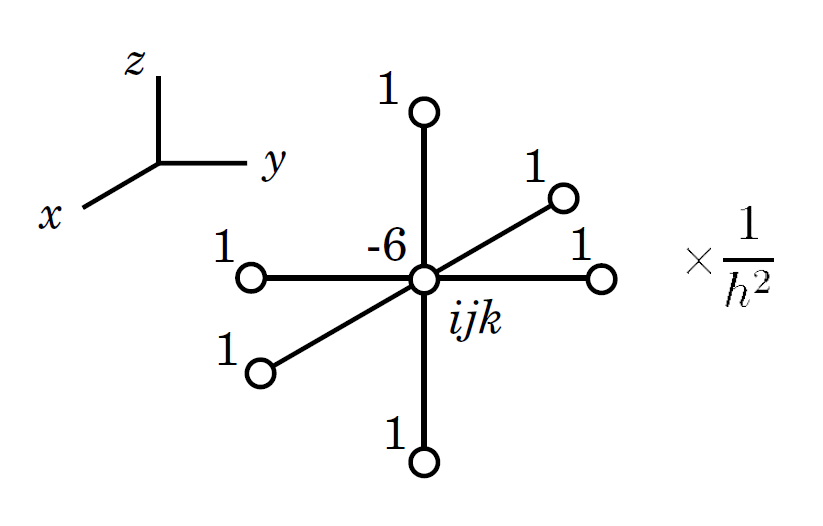
\includegraphics[width=\textwidth]{pictures/3/stencil7}
		\caption{7 points stencil}
		\label{fig:stencil7}
	\end{subfigure}
	\hfill
	\begin{subfigure}[b]{0.45\textwidth}
		\centering
		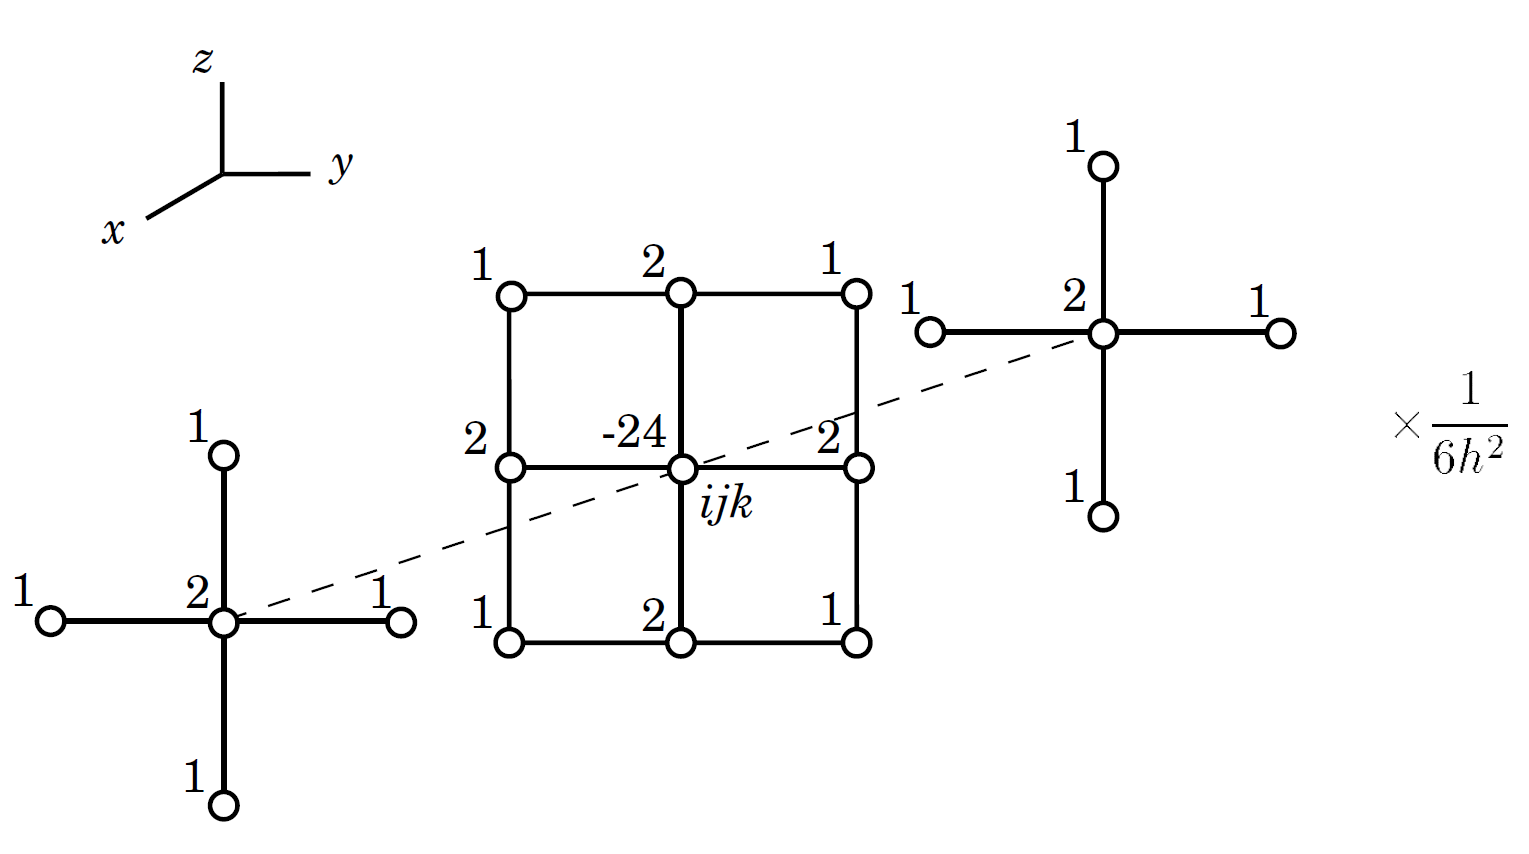
\includegraphics[width=\textwidth]{pictures/3/stencil19}
		\caption{19 points stencil}
		\label{fig:stencil19}
	\end{subfigure}
	\hfill
	\bigskip
	
	\begin{subfigure}[b]{0.45\textwidth}
		\centering
		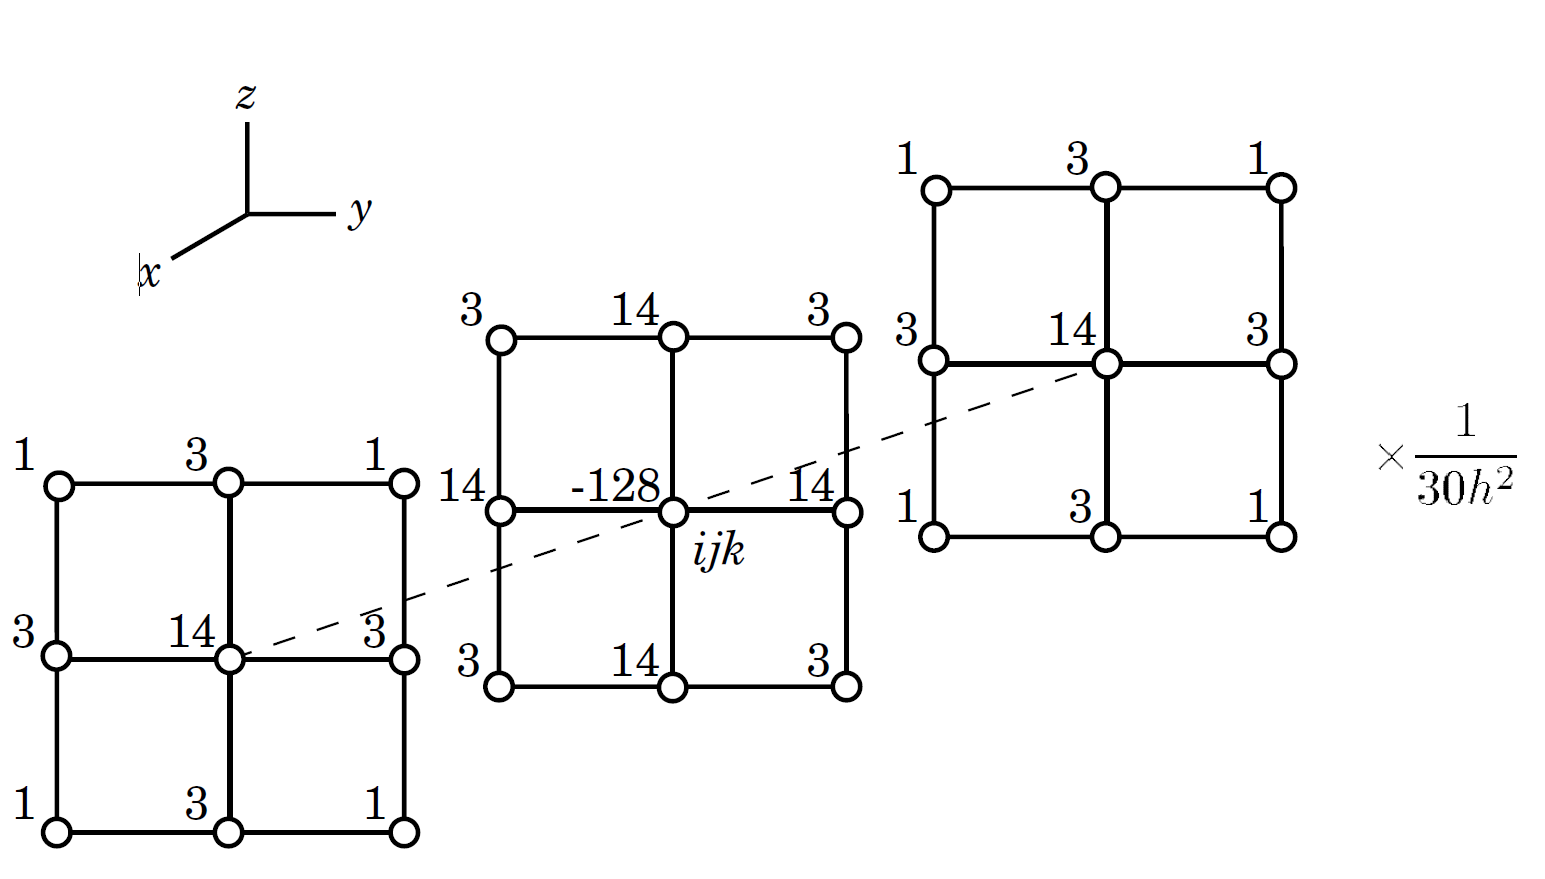
\includegraphics[width=\textwidth]{pictures/3/stencil27}
		\caption{27 points stencil}
		\label{fig:stencil27}
	\end{subfigure}
	\hfill
	
	\caption{CDS and HOC stencils described in William Spotz's dissertation. \cite{spotz1996hoc}}
	\label{fig:stencils}
\end{figure}


As Krotkiewski noted in his 2013 paper, those stencils are known as the general (non-separable) 3D convolution filters in computer graphics.\cite{krotkiewski2013efficient} 
% str. 5 rownanie 4




\subsection{Eigensolvers}
%TODO
Hereafter, and for the sake of simplicity, the sampled wavefunction flattened to a vector of N \times N \times N, \textbf{x} is defined to represent $\psi(x,y,z)$. What is left is calculating eigenvalues and eigenvectors using numerical methods. As stated before the time-independent Schr{\"o}dinger equation is:

\begin{equation}
	\hat{H} \psi(x,y,z) = E \psi(x,y,z)
\end{equation}

\noindent which is an eigenproblem,
%TODO
That is the transformation of wavefunction by Hamiltonian results in a scaled version. Because of discretization, the Hamiltonian can be treated as a matrix, and the wavefunction becomes a vector. To solve this for $E$, both sides of the equation are multiplied by $\psi^T(x,y,z).$

\begin{equation}
	\psi^T(x,y,z) \hat{H} \psi(x,y,z) = \psi^T(x,y,z) E \psi(x,y,z)
\end{equation}

\noindent note that $\psi^T(x,y,z)\psi(x,y,z)$ is a scalar, which means that E can be factored out on the right side

\begin{equation}
	\psi^T(x,y,z) \hat{H} \psi(x,y,z) = E(\psi^T(x,y,z) \psi(x,y,z))
\end{equation}

\noindent and both sides divided by also a scalar value of $\psi^T(x,y,z) \psi(x,y,z)$, which is an L2 norm of $\psi(x,y,z)$. After division, the equation becomes:

\begin{equation}
	E = \frac{\psi^T(x,y,z) \hat{H} \psi(x,y,z)}{\psi^T(x,y,z) \psi(x,y,z)}
\end{equation}

\noindent that is a Rayleigh's quotient, which is used in numerical calculations using computers since Vandergraft \cite{vandergraft1971} publication from 1971. Rayleigh's quotient can also be understood as a function that returns an eigenvalue when given a proper eigenvector.

\begin{equation}
	\lambda_i = R(\textbf{x}_i)
\end{equation}

\noindent

\subsubsection{Gradient descent}

Iterative methods were employed to solve the aforementioned quotient. The most basic algorithm, used for such tasks is gradient descent.\cite{gradient_descent} The algorithm idea is to have an initial guess of what the eigenvector might be. If no such information exists, an uniform random vector should be used. Then, the gradient of Rayleigh's quotient should be calculated. Since the gradient points in the direction where the function grows the fastest, and the algorithm tries to minimize the value, the gradient for the current $\textbf{x}$ iteration is calculated, negated, and multiplied by the learning rate. Thus, the next value of $\textbf{x}_{i+1}$ is:

\begin{equation}
	\textbf{x}_{i+1} = \textbf{x}_{i} - lr \cdot \nabla R(\textbf{x}_{i})
\end{equation}

\noindent, after which the check for convergence is made by checking if the L2 norm of the residue vector is greater than the assumed tolerance. Once the convergence criterion is satisfied or the maximum number of iterations is achieved, the procedure returns the eigenvalue and eigenvector. This algorithm enables the identification of the local minima of multivariate functions.

\subsubsection{Locally Optimal Block Preconditioned Conjugate Gradient}
%TODO
% Wikipedia, edit
% Locally Optimal Block Preconditioned Conjugate Gradient (LOBPCG) is a matrix-free method for finding the largest eigenvalues and the corresponding eigenvectors of a symmetric positive definite generalized eigenvalue problem. \cite{knyazew2001} Even though it is described as matrix-free, many implementations, such as one found in PyTorch, demand matrix operators.

Its implementations can be found in scientific modules such as SciPy \cite{scipy_lobpcg} and GPU-accelerated versions from PyTorch \cite{torch_lobpcg} and CuPyX \cite{cupy_lobpcg}.

\subsubsection{Steepest descent with optimal step}
%TODO
ŹRÓDŁO \cite{pgd}

The goal function is defined as
\begin{equation}
	\rho\left(\mathbf{x}, \bm{\lambda} \right) = \frac{\mathbf{x}^T\mathbf{A}\mathbf{x}}{\mathbf{x}^T\mathbf{x}} + \bm{\lambda}^T \mathbf{Y}^T \mathbf{x}, 
\end{equation}
where $\mathbf{Y}\in\mathbb{R}^{d \times k}$ contains orthogonal vectors defining the subspace orthogonal to the sought solution and $\bm{\lambda}\in\mathbb{R}^k$ is the vector of Lagrange multipliers.
Thus, the gradients read
\begin{equation}
	\nabla_{\mathbf{x}}\rho\left(\mathbf{x},\bm{\lambda}\right) = \frac{2}{\mathbf{x}^T\mathbf{x}}\left(\mathbf{A}-\frac{\mathbf{x}^T\mathbf{A}\mathbf{x}}{\mathbf{x}^T\mathbf{x}}\right)\mathbf{x} + \mathbf{Y}\bm{\lambda},
\end{equation}
\begin{equation}
	\nabla_{\bm{\lambda}}\rho\left(\mathbf{x},\bm{\lambda}\right) = \mathbf{Y}^T\mathbf{x}.
\end{equation}
The search direction for gradient descent is
\begin{equation}
	\mathbf{p}=-\left[\left(\nabla_{\mathbf{x}}\rho\left(\mathbf{x},\bm{\lambda}\right)\right)^T, \left(\nabla_{\bm{\lambda}}\rho\left(\mathbf{x},\bm{\lambda}\right)\right)^T\right]^T = \left[\mathbf{p}_{\mathbf{x}}^T,\mathbf{p}_{\bm{\lambda}}^T\right]^T.
\end{equation}

The goal as a function of the step size $\delta$ reads
\begin{equation}
	\rho\left(\mathbf{x}+\delta \mathbf{p}_{\mathbf{x}},\bm{\lambda}+\delta \mathbf{p}_{\bm{\lambda}}\right) = \frac{a_1+b_1\delta+c_1\delta^2}{a_2+b_2\delta+c_2\delta^2} + a_3+b_3\delta + c_3 \delta^2,
	\label{eq5}
\end{equation}
where
\begin{align*}
	a_1 &= \mathbf{x}^T\mathbf{A}\mathbf{x}, & \quad a_2 &= \mathbf{x}^T\mathbf{x}, & \quad a_3 &= \bm{\lambda}^T\mathbf{Y}^T\mathbf{x}, \\
	b_1 &= 2 \mathbf{p}_{\mathbf{x}}^T\mathbf{A}\mathbf{x}, & \quad b_2 &= 2\mathbf{p}_{\mathbf{x}}^T\mathbf{x}, & \quad b_3 &=  \mathbf{p}_{\bm{\lambda}} \mathbf{Y}^T \mathbf{x} + \bm{\lambda}\mathbf{Y}^T\mathbf{p}_{\mathbf{x}}, \\
	c_1 &= \mathbf{p}_{\mathbf{x}}^T \mathbf{A} \mathbf{p}_{\mathbf{x}}, & \quad c_2 &= \mathbf{p}_{\mathbf{x}}^T\mathbf{p}_{\mathbf{x}}, &  \quad c_3 &= \mathbf{p}_{\bm{\lambda}}^T\mathbf{Y}^T\mathbf{p}_{\mathbf{x}}.
\end{align*}
Minimization of \ref{eq5} w.r.t. $\delta$ leads to the $5$th order polynomial equation
\begin{equation}
	q_0 + q_1 \delta + q_2 \delta^2 + q_3 \delta^3 + q_4 \delta^4 +q_5 \delta^5 = 0,
\end{equation}
where the coefficients are:
\begin{align*}
	q_0 &= -a_1 b_2 + a_2 (b_1 + a_2 b_3),\\
	q_1 &= -2 a_1 c_2 + 2 a_2 (b_2 b_3 + c_1 + a_2 c_3),\\ 
	q_2 &= b_2^2 b_3 + b_2 c_1 - b_1 c_2 + 2 a_2 b_3 c_2 + 4 a_2 b_2 c_3, \\
	q_3 &= 2 (b_2 b_3 c_2 + b_2^2 c_3 + 2 a_2 c_2 c_3),\\
	q_4 &= c_2 (b_3 c_2 + 4 b_2 c_3),\\
	q_5 &= 2 c_2^2 c_3.
\end{align*}

which facilitates the calculation of the optimal step size.

\subsubsection{Adam}
%TODO

%\begin{aligned}
%	m_w^{(t+1)} = \beta_1 m_w^{(t)} + (1 - \beta_1) \nabla_w L^{(t)} \\
%	& v_w^{(t+1)} = \beta_2 v_w^{(t)} + (1 - \beta_2) (\nabla_w L^{(t)}) \\
%	& \hat{m_w} = frac{m_w^{(t+1)}}{1-\beta_1^t} \\
%	& \hat{v_w} = frac{v_w^{(t+1)}}{1-\beta_2^t} \\
%	& w^{(t+1)} = w^{(t)} - \eta frac{\hat{m_w}}{\sqrt{\hat{v_w}} + \epsilon}
%\end{aligne}
\cite{kingma_adam:_2017}

\subsection{Tools and techniques}

\subsubsection{Python}

\cite{mayavi}


\subsubsection{CuPy}

CuPy provides the functionality of NumPy and SciPy modules, offering GPU-accelerated computing with Python. It works on both Nvidia CUDA and AMD ROCm platforms. Its API is compatible with the aforementioned modules.\cite{cupy_overview}

CuPy also provides an easy way of implementing custom kernel functions. For example - taken from "Learn CUDA":\cite{learn_cuda}

\vspace{0.2cm}
\lstinputlisting[caption=Simple element-wise kernel, label=listing1, captionpos=b]{listings/3/listing1.py}
takes two arguments, x and y and the return value is stored in the variable z.

Also it is possible to use raw kernel functions. Raw kernels are used when one wants to define a custom kernel that executes CUDA source code. Using raw kernels allows for control of grid size, block size, shared memory size, and stream. An example of the raw kernel from CuPy docs\cite{cupy_raw_kernel}:

\vspace{0.2cm}
\lstinputlisting[caption=Example code of raw kernel that performs addition of two 2D arrays., label=listing2, captionpos=b]{listings/3/listing2.py}

Moreover, CuPy provided the TextureObject\cite{cupy_texture} and SurfaceObject\cite{cupy_surface}, allowing the CUDA textures and surfaces to be passed into the raw kernel. The relevance of this will be addressed in more depth in the next section. Also, the LOBPCG implementation from this module was used.\cite{cupy_lobpcg}


\subsubsection{CUDA}

In this work, we meet the case of data parallelism\cite{cheng2014professional}, which is a situation where calculation time might benefit when many data items are operated at the same time. The CUDA approach for such problems is to provide each thread with equal parts of data so that every thread can work on its part simultaneously.
%TODO BERGMAN NOTED! change this paragraph
An important issue with parallel computation has been raised by members of high performance computing (HPC) community. Krotkiewski noted, the \textit{flop to byte ratio} (F2B), defined as floating-point operations per second (FLOPs) divided by the available memory bandwith (in bytes per second) is a recognized challenge in high performance computing. It is especially important in algorithms that characterize in high memory utilization compared to the number of arithmetic instructions done. This puts pressure on scientists to design algorithms efficient not only from computational, but also space complexity.\cite{krotkiewski2013efficient}

\vspace{0.2cm}

\begin{table}[!ht]
	\centering
	\caption{Comparison of FLOP, Memory Bandwidth, and FLOP-to-Byte Ratio for NVIDIA GPUs}
	\label{tab:gpu-comparison}
	\resizebox{\textwidth}{!}{%
		\begin{tabular}{|l|c|c|c|}
			\hline
			\textbf{GPU Model}         & \textbf{FLOP (TFLOPS)} & \textbf{Memory Bandwidth (GB/s)} & \textbf{FLOP-to-Byte Ratio (FLOP/byte)} \\ \hline
			NVIDIA Tesla C2050         & 1.03                   & 144                              & 7.15                                    \\ \hline
			NVIDIA RTX A4000           & 19.2                   & 448                              & 42.9                                    \\ \hline
			NVIDIA TITAN RTX           & 16.3                   & 672                              & 24.2                                    \\ \hline
			NVIDIA GeForce RTX 4090    & 82.6                   & 1,010                            & 81.8                                    \\ \hline
			
		\end{tabular}%
	}
	\smallskip
	\small \textit{Source}: Own elaboration based on techpowerup.com publications\cite{techpowerup1}\cite{techpowerup2}\cite{techpowerup3}
\end{table}

Since the publication of Krotkiewki's findings, the problem only was exacerbated. The NVIDIA Tesla C2050 mentioned in his article has half of F2P compared to it's current successor, NVIDIA RTX A4000. Moreover, the cards utilized in this work were characterized by even higher F2P, further highlighting the growing disparity between computational power and memory bandwidth.
% tutaj wjezdza Akhtar i moja implementacja
\vspace{0.2cm}
\lstinputlisting[caption=Simple element-wise kernel, label=listing1, captionpos=b]{listings/3/listing1.py}
takes two arguments, x and y and the return value is stored in the variable z.

CUDA offers 

Raw kernels were written using the technique described by Akhtar et al.\cite{akhtar2018efficient}. and Krotkiewski \cite{krotkiewski2013efficient}


% TODO opisać texturę i surface i guess
% TODO opisać benchmark obliczenia numerycznego

\cite{learn_cuda}
\cite{cheng2014professional}





	
	\section{Results}

\subsection{Application of the new method}
%% Apply your method to relevant problems or case studies.

\subsubsection{Hamiltonian}

 The listing for 7-point stencil is presented in Listing 4. The boundary conditions were implemented to set the memory boundaries to zero explicitly. It utilizes the textures and surfaces as mentioned in Akhtar's article \cite{akhtar2018efficient}. Stencils of higher order were implemented in the same fashion. In Figure \ref{fig:laplacian}, a sample result of the Laplacian acting on $e^{-\sqrt{x^2+y^2+z^2)}}$ was presented.

\vspace{0.2cm}
\lstinputlisting[caption=Listing of Laplace operator., label=listing4, captionpos=b]{listings/4/listing4.py}

\begin{figure}[h]
	\centering
	\includegraphics[width=\textwidth]{pictures/4/wykres2.png}
	\caption{Plot of the Laplacian operating on $e^{-\sqrt{x^2+y^2+z^2	}}$ projected into z-axis. Source: Own elaboration}
	\label{fig:laplacian}
\end{figure}

The potential operator was also implemented utilizing efficient memory access patterns, as presented in Listing 5. The singularity of $\frac{1}{r}$ was resolved by introducing a parameter eps, which bounds the potential values above $\frac{1}{\sqrt{eps}}$, reducing numerical errors. The value of eps in this work was set to 100, limiting the potential to 10 a.u. This value was determined experimentally by searching for the optimal power of ten.
\newpage

\vspace{0.2cm}
\lstinputlisting[caption=Listing of potential operator., label=listing5, captionpos=b]{listings/4/listing5.py}

The result of implemented potential on a vector of one was presented in the Figure \ref{fig:potential}

\begin{figure}[h]
	\centering
	\includegraphics[width=\textwidth]{pictures/4/wykres1.png}
	\caption{Plot showing the potential energy in X axis. Source: Own elaboration}
	\label{fig:potential}
\end{figure}

Both operators are utilized in the Hamiltonian Python class, which provides the functionality of the matvec() function, which operates with Hamiltonian on a vector, and matmat(), which operates with Hamiltonian on a matrix. Those functions, as well as shape attribute are required to instantiate a CuPy Operator class with Hamiltonian. Methods pre() and post() are responsible for changing the mesh grid of shape $(N x N x N)$ to a vector of size $(N^3, 1)$.


\vspace{0.2cm}
\lstinputlisting[caption=Listing of Hamiltonian class., label=listing6, captionpos=b]{listings/4/listing6.py}


\subsubsection{Goal function and gradient class}

The equations presented in section 3.4 could be used as a general case for goal function. Thus, they were implemented as goal function class, with listing as follows:

\vspace{0.2cm}
\lstinputlisting[caption=Goal function class, label=listing7, captionpos=b]{listings/4/listing7.py}

This separates the responsibilities of representing the state of a wavefunction from calculations made on it by minimizing algorithms and returns the values of gradient and objective function. GoalGradient has two dependencies: A stands for the Hamiltonian operator object, while Y is the matrix containing previous wavefunctions from previous calculations. Y should be set to None during the first energy value computation.

The validation of both the Hamiltonian operator as well as GoalGradient class, according to the advice obtained during consultations \cite{SytySienkiewicz}, was through inputting it with a known wavefunction, which is described in the Comparative Analysis section.

\vspace{0.2cm}
\lstinputlisting[caption=Exemplary wavefunction implementation, label=listing8, captionpos=b]{listings/4/listing8.py}

The function constructs an \textit{ansatz} with the appropriate spatial extent (in hydrogen radii) and grid density, defined by the parameter $N$. These parameters must match those of the Hamiltonian class to ensure proper functioning.

\newpage

\subsection{Minimizing algorithms implementations}
\subsubsection{Gradient descent}

\vspace{0.2cm}
\lstinputlisting[caption=Gradient descent function implementation, label=listing9, captionpos=b]{listings/4/listing9.py}

\subsubsection{Adam}

\vspace{0.2cm}
\lstinputlisting[caption=Adam function implementation, label=listing10, captionpos=b]{listings/4/listing10.py}

\subsection{Comparative analysis}
%% Compare the results of the new method with those of existing methods. Use graphs, tables, or figures to illustrate differences in performance, accuracy, or computational efficiency.

\subsubsection{Hydrogen ground state validation}

The first step in validating the method was placing the known \textit{ansatz} functions in gradient algorithms to check whether they return correct values on the first step. This proves whether the Hamiltonian implementation and goal function class are correct. Wavefunction from the Listing \ref{listing8} was used for the ground state. Other \textit{ansatz} were implemented in the same fashion, according to formulas presented in Chapter 2.1. Table \ref{tab:stencil-comparison-ground-state-values} presents a summary of the obtained results.

\begin{table}[!ht]
	\centering
	\caption{Comparison ground state energies of hydrogen after first step. Analytically obtained value: -0.5}
	\label{tab:stencil-comparison-ground-state-values}
	\small % Adjust font size for the table
	\begin{tabular}{|l|c|c|c|}
		\hline
		\textbf{Stencil type} & \textbf{Gradient descent} & \textbf{Adam} & \textbf{LOBPCG} \\ \hline
		7-point               & -0.4954987                & -0.4941386    & -0.49549726 \\ \hline
		19-point              & -0.4963384                & -0.4957334    & -0.49633817 \\ \hline
		27-point              & -0.4963269                & -0.4956166    & -0.49632594 \\ \hline
	\end{tabular}
	
	\smallskip
	\small \textit{Source}: Own elaboration
\end{table}

This proves the objective function returns approximately correct results utilizing the Hamiltonian operator with implemented stencils. Next up, the methods were inputted with a random vector to check whether the algorithms converge to correct values of ground state energy, while the time and number of iterations for each Laplacian stencils were measured. Obtained results were summarized in Table \ref{tab:algorithm-comparison-ground-state}.

\begin{table}[!ht]
	\centering
	\caption{Value, time, and iterations of each algorithm with different stencil types}
	\label{tab:algorithm-comparison-ground-state}
	\small
	% Specify a width (e.g. \textwidth) and keep height as '!'
	\resizebox{\textwidth}{!}{
		\begin{tabular}{|l|ccc|ccc|ccc|}
			\hline
			& \multicolumn{3}{c|}{\textbf{Gradient descent}} 
			& \multicolumn{3}{c|}{\textbf{Adam}} 
			& \multicolumn{3}{c|}{\textbf{LOBPCG}} \\ 
			& \multicolumn{3}{c|}{[$l_r=10^{-5}$, $tol=10^{-5}$]} 
			& \multicolumn{3}{c|}{[$l_r=10^{-5}$, $tol=10^{-5}$]} 
			& \multicolumn{3}{c|}{[$tol=10^{-5}$]} \\ \hline
			\textbf{Stencil:} & \textit{Value} & \textit{Iterations} & \textit{Time} 
			& \textit{Value} & \textit{Iterations} & \textit{Time} 
			& \textit{Value} & \textit{Iterations} & \textit{Time} \\
			\hline
			7-point    & -0.49593 & 8431 & 775s & -0.49248 & 896 & 95s 
			& -0.49600 & 1246 & 205s \\ \hline
			19-point   & -0.49661 & 8422 & 755s & -0.49512 & 797 & 88s 
			& -0.49667 & 712 & 116s \\ \hline
			27-point   & -0.49661 & 8417 & 779s & -0.49485 & 813 & 88s 
			& -0.49667 & 756 & 125s \\ \hline
		\end{tabular}
	}
	\smallskip
	\small \textit{Source}: Own elaboration
\end{table}


\subsubsection{Hydrogen excited states validation}

Once the algorithms' ability to calculate the ground state of hydrogen has been analyzed, the next step was to check which algorithms perform best in calculating excited states of hydrogen. Due to the long convergence time, this section did not test gradient descent. In all analyses, 19-point stencils were used. Moreover, due to the bigger orbitals calculated, the extent of the considered cube had to be raised to <-30,30> hydrogen radii, described with $301 \times 301 \times 301$ grid. Adam utilized learning rate of $10^{-5}$ for x gradient, while the learning rate for lambda has been set to $10^{-3}$, and tolerance $10^{-5}$, while LOBPCG was inputted with tolerance of $10^{-5}$. This setup calculated the first three energy values while measuring time and iterations. The values obtained are presented in Table \ref{tab:adam-excited}:

\begin{table}[!ht]
	\centering
	\caption{Excited hydrogen states calculated using Adam and LOBPCG}
	\label{tab:adam-excited}
	\small % Adjust font size for the table
	\begin{tabular}{|c|c|c|c|}
		\hline
		\textbf{Expected result} & \textbf{LOBPCG} & \textbf{Adam} \\ \hline
		-0.125              & -0.12524    & -0.12507 \\ \hline
		-0.125              & -0.12524    & -0.06315 \\ \hline
		-0.125              & -0.12514    & -0.11625 \\ \hline
	\end{tabular}
	\smallskip
	
	\small \textit{Source}: Own elaboration
\end{table}

Due to changes in grid size, LOBPCG calculating four values at once took less time than calculating ground state alone (just 88 seconds), while Adam sequentially calculated the values and needed more time - the whole calculation needed 2636 seconds and usually ended only once maximum iteration value of 10000 was reached. Moreover, the second value did not converge over the constrained space -- the second value, which later became a constraint, also most probably added an error to the third value. 

Further investigation was done with Adam algorithm. The hyperparameter space of learning rate for $x$ and $\lambda$ was searched, and the results were presented in Table \ref{tab:hyperparameter-search}. The encountered problem was that with a too low a learning rate of $\lambda$ ($LR_\lambda$) compared to a learning rate of $x$ ($LR_x$) with each step, the constraint was largely ignored until reaching the ground state energy. On the other hand, too high values of ($LR_\lambda$) created oscillations, which made the convergence check unable to stop the algorithm. The only solution found yet, with both learning rates low enough, and correct values were reached after 30000 iterations (the whole calculation took 5449 seconds) due to maximum iteration check. The results for these parameters are summarized in Table \ref{tab:adam-optimized}.

\renewcommand{\arraystretch}{1.5}
\begin{table}[h]
	\centering
	\caption{Hyperparameter space search}
	\label{tab:hyperparameter-search}
	\small
	\begin{tabular}{|c|>{\centering\arraybackslash}p{3cm}|>{\centering\arraybackslash}p{3cm}|>{\centering\arraybackslash}p{3cm}|>{\centering\arraybackslash}p{3cm}|}
		
		\hline
		\diagbox[dir=SE]{$LR_\lambda$}{$LR_x$} & $10^{-3}$ & $10^{-4}$ & $10^{-5}$  & $10^{-6}$\\ 
		\hline
		$10^{-2}$ & always converges to -0.5 & $\lambda$ oscillations prevent convergence  & $\lambda$ oscillations prevent convergence & $\lambda$ oscillations prevent convergence  \\ 
		\hline
		$10^{-3}$ & always converges to -0.5 & always converges to -0.5 & $\lambda$ oscillations prevent convergence & \textbf{correct results, long convergence}  \\ 
		\hline
		$10^{-4}$ & always converges to -0.5 & always converges to -0.5 & always converges to -0.5 & always converges to -0.5  \\ 
		\hline
	\end{tabular}
	\smallskip
	
	\small \textit{Source}: Own elaboration
\end{table}


\begin{table}[!ht]
	\centering
	\caption{Adam with hyperparameters: $LR_\lambda=10^-3$, $LR_x = 10^-6$, $max-iter = 30000$}
	\label{tab:adam-optimized}
	\small % Adjust font size for the table
	\begin{tabular}{|c|c|c|c|}
		\hline
		\textbf{Expected result} & \textbf{Adam}  \\ \hline
		-0.125    & -0.11436 \\ \hline
		-0.125      & -0.12496 \\ \hline
		-0.125     & -0.12489 \\ \hline
	\end{tabular}
	\smallskip
	
	\small \textit{Source}: Own elaboration
\end{table}

LOBPCG was unable to calculate more than 12 eigenstates, their energies being largely close to expected. Further increasing the number was not feasible due to the larger space needed for the correct representation of higher-energy orbitals at the cost of precision, and it used up all VRAM of RTX 4090. The eigenvectors obtained during calculations were visualized using the Mayavi module, as presented in Figures \ref{fig:isosurfaces-cross-section} - \ref{fig:3-orbitals}.

\subsection{Discussion of results}

The implementation of the Hamiltonian operator was proved to be correct. From the implemented stencils, the best values for ground state energy in the number of iterations, time, and precision of the results were obtained using a 19-point stencil. All the metrics of a 27-point stencil were close to those of a 19-point stencil but slightly worse. The 7-point stencil performed the worst of all methods to implement Laplacian. Most probably, the 19-point stencil's performance can be attributed to the way it balances the computational and memory read constraints of the GPU.

During ground state calculations, the fastest converging algorithm in terms of iterations was LOBPCG, which converged in 712 iterations. One iteration of LOBPCG took longer than the iteration of Adam; thus, the fastest converging algorithm in terms of time was Adam utilizing a 19-point stencil, which converged in 88 seconds. The same time result was obtained for the 27-point stencil Adam implementation. The worst converging algorithm was gradient descent.

Both Adam and LOBPCG correctly calculated the excited hydrogen states, although Adam needed more iterations and a more specific search of the hyperparameters. Overall, the first four eigenstates were calculated using Adam, and the first twelve using LOBPCG. The obtained wavefunctions upon visual inspection proved to be similar to the expected results, although wavefunctions obtained with Adam showed some deformation, especially the 2p orbitals.

\begin{figure}[h]
	\centering
	\begin{subfigure}[b]{0.45\textwidth}
		\centering
		\includegraphics[width=\textwidth]{pictures/4/a2sp.png}
		\caption{2s orbital calculated with Adam, cross-section}
		\label{fig:a2sp}
	\end{subfigure}
	\hfill
	\begin{subfigure}[b]{0.45\textwidth}
		\centering
		\includegraphics[width=\textwidth]{pictures/4/l2sp.png}
		\caption{2s orbital calculated with LOBPCG, cross-section}
		\label{fig:l2sp}
	\end{subfigure}
	\hfill
	
	\bigskip
	
	\begin{subfigure}[b]{0.45\textwidth}
		\centering
		\includegraphics[width=\textwidth]{pictures/4/l3sp.png}
		\caption{3s orbital calculated with LOBPCG, cross-section}
		\label{fig:l3sp}
	\hfill
	\end{subfigure}
	\caption{Radial nodes visible in both Adam and LOBPCG calculated wavefunctions. Source: Own elaboration}
	\label{fig:isosurfaces-cross-section}
\end{figure} 

\begin{figure}[ht!]
	\centering
	\begin{subfigure}[b]{0.45\textwidth}
		\centering
		\includegraphics[width=\textwidth]{pictures/4/a1s.png}
		\caption{1s orbital calculated with Adam}
		\label{fig:a1s}
	\end{subfigure}
	\hfill
	\begin{subfigure}[b]{0.45\textwidth}
		\centering
		\includegraphics[width=\textwidth]{pictures/4/a2s.png}
		\caption{2s orbital calculated with Adam}
		\label{fig:a2s}
	\end{subfigure}
	\hfill
	
	\bigskip
	
	\begin{subfigure}[b]{0.45\textwidth}
		\centering
		\includegraphics[width=\textwidth]{pictures/4/a2p.png}
		\caption{2p orbital calculated with Adam}
		\label{fig:a2px}
	\end{subfigure}
	\hfill
	\begin{subfigure}[b]{0.45\textwidth}
		\centering
		\includegraphics[width=\textwidth]{pictures/4/2pieczarka.png}
		\caption{3s/2p hybrid orbital calculated with Adam}
		\label{fig:a2p}
	\end{subfigure}
	\hfill
	
	\caption{Orbitals calculated with Adam, isosurface on 0.95 probability. Source: Own elaboration}
	\label{fig:adam-isosurfaces}
\end{figure} 

\begin{figure}[h]
	\centering
	\begin{subfigure}[b]{0.45\textwidth}
		\centering
		\includegraphics[width=\textwidth]{pictures/4/l1s.png}
		\caption{1s orbital calculated with LOBPCG}
		\label{fig:l1s}
	\end{subfigure}
	\hfill
	\begin{subfigure}[b]{0.45\textwidth}
		\centering
		\includegraphics[width=\textwidth]{pictures/4/l2s.png}
		\caption{2s orbital calculated with LOBPCG}
		\label{fig:l2s}
	\end{subfigure}
	\hfill
	
	\bigskip
	
	\begin{subfigure}[b]{0.45\textwidth}
		\centering
		\includegraphics[width=\textwidth]{pictures/4/l2p.png}
		\caption{One of three 2p orbitals calculated with LOBPCG}
		\label{fig:l2p}
	\end{subfigure}
	\hfill
	\begin{subfigure}[b]{0.45\textwidth}
		\centering
		\includegraphics[width=\textwidth]{pictures/4/l2px.png}
		\caption{One of three 2p orbitals calculated with LOBPCG}
		\label{fig:l2px}
	\end{subfigure}
	\hfill
	\caption{Isosurfaces of the N=1 and N=2 orbitals, calculated using the LOBPCG method, visualized at the 0.95 probability threshold. Source: Own elaboration}
	\label{fig:1-2-orbitals}
\end{figure} 

\begin{figure}[t]
	\centering
	\begin{subfigure}[b]{0.45\textwidth}
		\centering
		\includegraphics[width=\textwidth]{pictures/4/l3s.png}
		\caption{3s orbital calculated with LOBPCG}
		\label{fig:l3s}
	\end{subfigure}
	\hfill
	\begin{subfigure}[b]{0.45\textwidth}
		\centering
		\includegraphics[width=\textwidth]{pictures/4/l3p.png}
		\caption{One of three 3p orbitals calculated with LOBPCG}
		\label{fig:l3p}
	\end{subfigure}
	\hfill
	
	\bigskip
	
	\begin{subfigure}[b]{0.45\textwidth}
		\centering
		\includegraphics[width=\textwidth]{pictures/4/l3px.png}
		\caption{One of three 3p orbitals calculated with LOBPCG}
		\label{fig:l3px}
	\end{subfigure}
	\hfill
	\begin{subfigure}[b]{0.45\textwidth}
		\centering
		\includegraphics[width=\textwidth]{pictures/4/l3pz.png}
		\caption{One of three 3p orbitals calculated with LOBPCG}
		\label{fig:l3pz}
	\end{subfigure}
	\hfill
	
	\bigskip
	
	\begin{subfigure}[b]{0.45\textwidth}
		\centering
		\includegraphics[width=\textwidth]{pictures/4/l3d.png}
		\caption{}
		\label{fig:l3d}
	\end{subfigure}
	\hfill	
	\begin{subfigure}[b]{0.45\textwidth}
		\centering
		\includegraphics[width=\textwidth]{pictures/4/l3d3.png}
		\caption{}
		\label{fig:l3d3}
	\end{subfigure}
	\hfill	
	\caption{Isosurfaces of the N=3 orbitals, calculated using the LOBPCG method, visualized at the 0.95 probability threshold. Source: Own elaboration}
	\label{fig:3-orbitals}
\end{figure} 
	
	\section{Conclusion}

\subsection{Summary of results}

%Targets of this work that were achieved:
%
%- three Laplace' operators were implemented using finite difference methods, with 7-point, 19-point and 27-point stencil
%
%- the trial ansatz of hydrogen as in Kołos' book were discretized and implemented as CuPy functions successfully
%
%- a goal function class to provide functions that describe the current state of the wavefunction was developed successfully
%
%- the trial ansatz was used to prove the correctness of goal function classes
%
%- two minimizing algorithms: gradient descent, Adam were implemented
%
%- gradient descent and Adam correctness was proven using trial ansatz
%
%- ground state energies from random vector were obtained successfully using gradient descent and Adam
%
%- although Adam reproduced the values from random vector, the method took very long time, was prone to oscillations
%
%- implementation of PGD failed to bring results
%
%- LOBPCG CuPy implementetion was successfully applied to calculate 12 quantum states of hydrogen
%
%- for calculating the ground state of hydrogen, the fastest results were obtained using Adam, but the most gradient descent with low learning rate proved to be more precise
%
%- the best results for obtaining excited hydrogen states is LOBPCG with 27-point stencil

In this work, several significant milestones were achieved in the numerical computation of hydrogen wavefunctions using the finite difference method (FDM). Three Laplace operators were successfully implemented using 7-point, 19-point, and 27-point stencils. These implementations provided increasingly accurate approximations of the Laplacian, critical for modeling the Hamiltonian operator in Schrödinger’s equation.

The trial ansatz for the hydrogen wavefunction, as described in Kołos’ book, was discretized and implemented as CuPy functions. Additionally, a dedicated goal function class was developed to describe and evaluate the state of the wavefunction, providing the foundation for optimization algorithms. The correctness of this implementation was validated using the trial ansatz.

Two optimization algorithms, gradient descent and Adam, were implemented to minimize Rayleigh's quotient and determine the ground state energy. Both algorithms were tested and confirmed to produce correct results using the trial ansatz. Using random initial wavefunctions, ground state energies were successfully obtained. However, while Adam reproduced the expected results, it was prone to oscillations and required significantly more computational time compared to gradient descent. For low learning rates, gradient descent proved more precise than Adam.

The implementation of the Perturbed Gradient Descent (PGD) method did not yield successful results, primarily due to challenges in its implementation. In contrast, the Locally Optimal Block Preconditioned Conjugate Gradient (LOBPCG) method, implemented in CuPy, was successfully used to compute 12 quantum states of hydrogen. For excited states, LOBPCG coupled with the 27-point stencil yielded the best results. This highlights the method’s efficiency and precision for higher-energy states.

\subsection{Conclusions and implications}

%- the implementations proved the theory was correct
%
%- finite difference method is well enough method for approximating Laplacian part of hamiltonian operator, to calculate the hydrogen states properly
%
%- current customer graphics card are capable not only of small educational tasks, such as Schr{\"o}dinger equation in 2D, but also bigger 3D systems, such as atom states
%
%- the calculations were done simultaneously on 12 wave functions each discretized on a cube with 80 bohr radius edge length. This means that systems of size about ~1000 bohr radius, or 51nm can be modelled using the same method and hardware.
The outcomes of this study validate the theoretical basis for using FDM to approximate the Laplacian in quantum mechanical problems. The method accurately modeled the hydrogen wavefunction and its energy states, demonstrating the viability of GPU-based computations for solving Schrödinger's equation in 3D systems.

This work also highlights the computational power of modern consumer-grade graphics cards. The calculations, performed simultaneously on 12 wavefunctions, each discretized on a cubic grid with an edge length of 80 Bohr radii, suggest that systems up to approximately 1000 Bohr radii (~51 nm) could be modeled with the same approach and hardware. These findings indicate that FDM can scale effectively to model larger quantum systems, bridging the gap between educational demonstrations and research-level applications.

\subsection{Future work}

%- the hyperparameters of Adam require refining, and the algorithm itself might be improved
%
%- the PGD method might be a better solution than Adam, if the problems with implementation are overcomed
%
%- the goal function class might benefit from caching the results, thus reducing numerical complexity
%
%method can be further developed by:
%
%- adding a UI that is consistent with existing quantum chemistry packages
%
%- adding options as external potential
%
%- hamiltonian has to be checked for potential of optimization, especially space complexity
%
%- a C++/C CUDA implementation might provide even better results, especially the ability to decide when the memory is freed
%
%- current computers frequently have bigger RAM than GPU's VRAM, as well as faster than ever SSDs - there might be a space for improvement by storing some of the data on either of those spaces
%
%- calculations of helium atom and hydrogen molecule should be next steps in development of FDM methods for quantum chemistry
Several avenues for future development arise from this research. The Adam optimizer, while functional, requires hyperparameter refinement to improve its efficiency and stability. Further improvements to the algorithm itself may reduce its susceptibility to oscillations. Additionally, addressing the implementation challenges in PGD could make it a viable alternative to Adam, particularly for systems requiring higher stability.

The goal function class could benefit from caching intermediate results, potentially reducing numerical complexity and improving performance. Furthermore, integrating a user interface aligned with existing quantum chemistry packages would enhance usability. Adding features such as external potential options and optimizing the Hamiltonian's space complexity could make the framework more versatile and efficient.

A dedicated C++/CUDA implementation may further enhance performance, particularly by providing more control over memory management. Given the disparity between system RAM and GPU VRAM in modern computers, and the increasing speed of SSDs, storing intermediate data in these memory spaces could improve scalability and efficiency.

Finally, extending this method to more complex systems, such as the helium atom and the hydrogen molecule, is a natural progression. These steps would deepen the applicability of FDM in quantum chemistry and expand its role in computational physics research.
	
	\begin{singlespace} % Interlinia 1
		\addcontentsline{toc}{section}{References}
		\printbibliography[title=References]
		% Np. type=book / nottype=online w przypadku rozdziału na rodzaje
%		\printbibliography[title=References: articles, type=article]
%		\printbibliography[title=References: books, type=book]
		%\printbibliography[title=References: phdthesis, type=phdthesis]
		\sloppy % Łamie URL, tak żeby zgadzały się z ustalonymi marginesami strony
%		\printbibliography[title=References: online sources, type=online]
		% Rozdział bibliografii na dwie sekcje daje ostrzeżenie z zachętą do rozdzielenia numeracji
	\end{singlespace}
	
	\newpage
	\begin{singlespace} % Interlinia 1
		\addcontentsline{toc}{section}{List of figures}
		\renewcommand{\listfigurename}{List of Figures}
		\listoffigures
	\end{singlespace}
	
	\newpage
	\begin{singlespace} % Interlinia 1
		\addcontentsline{toc}{section}{List of Tables}
		\renewcommand{\listtablename}{List of Tables}
		\listoftables
	\end{singlespace}
	
	\newpage
	\begin{singlespace} % Interlinia 1
		\addcontentsline{toc}{section}{List of Listings}
		\renewcommand{\lstlistlistingname}{List of Listings}
		\lstlistoflistings
	\end{singlespace}
	
	\section{Appendices}
\subsection{Code}

The code developed during this master thesis is available upon request. For access contact me directly via email at blaz.tez@gmail.com. The associated GitHub repository URL is \url{https://github.com/blazejtez/qc}.

\subsection{Detailed proofs}
\subsubsection{7-point stencil}
Derivation begins with the Laplacian operator:
\begin{equation}
	\Delta = \frac{\partial^2}{\partial x^2} + \frac{\partial^2}{\partial y^2} + \frac{\partial^2}{\partial z^2}
	\label{eq1}
\end{equation}
The derivative can be approximated as a difference quotient of:
\begin{equation}
	\frac{df(x)}{dx} \approx \frac{f(x)-f(x-h)}{h}
	\label{eq2}
\end{equation}
as well as a difference quotient from the other side:
\begin{equation}
	\frac{df(x+h)}{dx} \approx \frac{f(x+h)-f(x)}{h}
	\label{eq3}
\end{equation}
where h is a grid spacing.
To calculate the second derivative we use formula \ref{eq3}:
\begin{equation}
	\frac{d^2f(x)}{dx^2} = \frac{df(x)}{dx} \frac{df(x)}{dx} = \frac{d}{dx} \frac{f(x+h)-f(x)}{h}
\end{equation}

\begin{equation}
	\frac{d}{dx} \frac{f(x+h)-f(x)}{h} = \frac{1}{h} \frac{d}{dx}(f(x+h)-f(x)) = \frac{1}{h} (\frac{df(x+h)}{dx} - \frac{df(x)}{dx})
\end{equation}

\noindent And thus we can substitute into \ref{eq2} and \ref{eq3}:
\begin{equation}
	\frac{d^2f(x)}{dx^2} = \frac{1}{h} (\frac{f(x+h)-f(x)}{h} - \frac{f(x)-f(x-h)}{h}) = \frac{1}{h^2} (f(x+h)-f(x)-(f(x)-f(x-h))) 
\end{equation}
\begin{equation}
	= \frac{1}{h^2} (f(x+h)-f(x)-f(x)+f(x-h)) = \frac{1}{h^2} (f(x+h)+f(x-h)-2f(x))
\end{equation}
Calculations for y and z will be similar. As long as h is the same in any dimension, we can substitute this into \ref{eq1}:
\begin{equation}
	\Delta = \frac{1}{h^2} (f(x+h)+f(x-h)-2f(x)) + \frac{1}{h^2} (f(y+h)+f(y-h)-2f(y)) + \frac{1}{h^2} (f(z+h)+f(z-h)-2f(z))
\end{equation}
\begin{equation}
	\Delta = \frac{1}{h^2} (f(x+h)+f(x-h)-2f(x) + f(y+h)+f(y-h)-2f(y) + f(z+h)+f(z-h)-2f(z))
\end{equation}
For point in space f(x,y,z), we derive 7-point stencil:

\begin{equation}
	\begin{aligned}
		\Delta = \frac{1}{h^2} \Big( 
		& f(x+h, y, z) + f(x-h, y, z) + f(x, y+h, z) \\
		& + f(x, y-h, z) + f(x, y, z+h) + f(x, y, z-h) \\
		& - 6f(x, y, z) 
		\Big)
	\end{aligned}
\end{equation}
%
%\subsubsection{Integrating the expectation value of the potential energy operator}
%\begin{equation}
%	\int_{-\infty}^{+\infty} \int_{-\infty}^{+\infty} \int_{-\infty}^{+\infty} 
%	x^k y^l z^m e^{-p (x^2+y^2+z^2)} \frac{1}{\sqrt{x^2+y^2+z^2}} x^k y^l z^m e^{-p(x^2+y^2+z^2)}
%	dx dy dz
%\end{equation}
%
%\noindent Substitute:
%
%\begin{align*} 
%	r^2 &=  x^2+y^2+z^2 \\ 
%	r &=  \sqrt{x^2+y^2+z^2} \\
%	x &= r \sin{\theta} \cos{\phi} \\
%	y &= r \sin{\theta} \sin{\phi} \\
%	z &= r \cos{\theta} \\
%	J &= r^2 \sin{\theta}
%\end{align*}
%
%\noindent Leads to:
%
%\begin{multline}
%	\int_{0}^{+\infty} \int_{0}^{2\pi} \int_{0}^{\pi} 
%	(r \sin{\theta} \cos{\phi})^k
%	(r \sin{\theta} \sin{\phi})^l
%	(r \cos{\theta})^m 
%	e^{-p r^2}
%	\\
%	(r \sin{\theta} \cos{\phi})^k
%	(r \sin{\theta} \sin{\phi})^l
%	(r \cos{\theta})^m
%	e^{-p r^2} 
%	\frac{1}{r}
%	r^2 \sin{\theta}
%	d\phi d\theta d r
%\end{multline}
%
%\noindent Reducing:
%
%\begin{equation}
%	\int_{0}^{+\infty} \int_{0}^{2\pi} \int_{0}^{\pi} 
%	(r \sin{\theta} \cos{\phi})^{2k}
%	(r \sin{\theta} \sin{\phi})^{2l}
%	(r \cos{\theta})^{2m}
%	e^{-2p r^2} 
%	r \sin{\theta}
%	d\phi d\theta d r
%\end{equation}
%
%\noindent Split the integrand into three functions:
%
%\begin{equation}
%	(r \sin{\theta} \cos{\phi})^{2k}
%	(r \sin{\theta} \sin{\phi})^{2l}
%	(r \cos{\theta})^{2m}
%	e^{-2p r^2} 
%	r \sin{\theta}
%\end{equation}
%
%\begin{equation}
%	r^{2k} \sin^{2k}{\theta} \cos^{2k}{\phi} 
%	r^{2l} \sin^{2l}{\theta}  \sin^{2l}{\phi} 
%	r^{2m} \cos^{2m}{\theta} 
%	e^{-2p r^2} 
%	r \sin{\theta}
%\end{equation}
%
%\begin{equation}
%	(r^{2k} r^{2l} r^{2m} e^{-2p r^2} r)
%	(\sin^{2k}{\theta}\sin^{2l}{\theta} \cos^{2m}{\theta}  \sin{\theta} )
%	(\cos^{2k}{\phi}   \sin^{2l}{\phi} )
%\end{equation}
%
%\begin{equation}
%	(r^{2(k+l+m)+1} e^{-2p r^2})
%	(\sin^{2(k+l)+1}{\theta}\cos^{2m}{\theta})
%	(\cos^{2k}{\phi}   \sin^{2l}{\phi} )
%\end{equation}
%From which derives:
%\begin{equation}
%	\int_{0}^{+\infty} r^{2(k+l+m)+1} e^{-2p r^2} d r
%	\int_{0}^{2\pi} \sin^{2(k+l)+1}{\theta}\cos^{2m}{\theta} d\theta
%	\int_{0}^{\pi} \cos^{2k}{\phi}   \sin^{2l}{\phi} d\phi
%\end{equation}
%Which using Mathematica is calculated as equal to:
%\begin{multline}
%	\frac{\Gamma \left(k+\frac{1}{2}\right) \Gamma \left(l+\frac{1}{2}\right) \Gamma \left(m+\frac{1}{2}\right) 2^{-k-l-m-2} p^{-k-l-m-1} \Gamma (k+l+m+1)}{\Gamma\left(k+l+m+\frac{3}{2}\right)} \\
%\end{multline}
%
%\subsubsection{Integrating the expectation value of the kinetic energy operator}
%\begin{equation}
%	\int_{-\infty}^{+\infty} \int_{-\infty}^{+\infty} \int_{-\infty}^{+\infty} 
%	x^k y^l z^m e^{-p (x^2+y^2+z^2)} \Delta x^k y^l z^m e^{-p(x^2+y^2+z^2)}
%	dx dy dz
%\end{equation}
%
%\noindent Simplify the integrand:
%\begin{equation}
%	x^k y^l z^m e^{-p (x^2+y^2+z^2)} \Delta x^k y^l z^m e^{-p(x^2+y^2+z^2)}
%\end{equation}
%
%\begin{equation}
%	(\frac{\partial^2}{\partial x^2} + \frac{\partial^2}{\partial y^2} + \frac{\partial^2}{\partial z^2})x^k y^l z^m e^{-p(x^2+y^2+z^2)}
%\end{equation}
%
%\noindent Split the integrand into three functions:
%\begin{equation}
%	\frac{\partial^2}{\partial x^2} x^k y^l z^m e^{-p(x^2+y^2+z^2)}
%\end{equation}
%
%\begin{equation}
%	\frac{\partial^2}{\partial y^2} x^k y^l z^m e^{-p(x^2+y^2+z^2)}
%\end{equation}
%
%\begin{equation}
%	\frac{\partial^2}{\partial z^2} x^k y^l z^m e^{-p(x^2+y^2+z^2)}
%\end{equation}
%
%\noindent Next calculate first second-order partial derivative:
%
%\begin{equation}
%	\frac{\partial^2}{\partial x} x^k y^l z^m e^{-p(x^2+y^2+z^2)}
%\end{equation}
%
%\begin{equation}
%	y^l z^m \frac{\partial^2}{\partial x^2} x^k e^{-p(x^2+y^2+z^2)}
%\end{equation}
%
%\begin{equation}
%	y^l z^m \frac{\partial^2}{\partial x^2} x^k e^{-px^2-py^2-pz^2}
%\end{equation}
%
%\begin{equation}
%	y^l z^m \frac{\partial^2}{\partial x^2} x^k e^{-px^2}e^{-py^2}e^{-pz^2}
%\end{equation}
%
%\begin{equation}
%	y^l z^m e^{-py^2}e^{-pz^2} \frac{\partial^2}{\partial x} x^k e^{-px^2}
%\end{equation}
%
%\noindent Which gives the value of first partial derivative:
%\begin{equation}
%	\frac{\partial^2\phi(x,y,z)}{\partial x^2} = y^l z^m e^{-py^2}e^{-pz^2}  \left(x^k (4 p^2 x^2 e^{-p x^2}-2 p e^{-p x^2})+(k-1) k x^{k-2} e^{-p x^2}-4 k p x^k e^{-p x^2}\right)
%\end{equation}
%
%\noindent Similarly, for the second mixed partial derivative, yields:
%
%\begin{equation}
%	x^k z^m e^{-px^2}e^{-pz^2} \frac{\partial^2}{\partial y^2} y^l e^{-py^2}
%\end{equation}
%
%\noindent Which gives the value of second partial derivative:
%\begin{equation}
%	\frac{\partial^2\psi(y)}{\partial y^2} =  x^k z^m e^{-px^2}e^{-pz^2} \left( z^m (4 p^2 z^2 e^{-p z^2}-2 p e^{-p z^2})+(m-1) m z^{m-2} e^{-p z^2}-4 m p z^m e^{-p z^2} \right)
%\end{equation}
%
%\noindent And the third yields:
%\begin{equation}
%	x^k y^l e^{-px^2}e^{-py^2} \frac{\partial^2}{\partial z^2} z^m e^{-pz^2}
%\end{equation}
%
%\noindent The result obtained with Mathematica:
%\begin{equation}
%	\frac{\partial^2\psi(z)}{\partial z^2} = x^k y^l e^{-px^2}e^{-py^2} \left( y^l (4 p^2 y^2 e^{-p y^2}-2 p e^{-p y^2})+(l-1) l y^{l-2} e^{-p y^2}-4 l p y^l e^{-p y^2}\right)
%\end{equation}
%
%\noindent Now the integral can be split into a sum of three integrals:
%
%\begin{equation}
%	I_1 = \psi \frac{\partial^2\psi(x,y,z)}{\partial x^2}
%\end{equation}
%\begin{equation}
%	I_2 = \psi \frac{\partial^2\psi(x,y,z)}{\partial y^2}
%\end{equation}
%\begin{equation}
%	I_3 = \psi \frac{\partial^2\psi(x,y,z)}{\partial z^2}
%\end{equation}
%
%Każda z nich była obliczana w analogiczny sposób:
%
%\begin{equation}
%	I_1 = \psi x^k y^l z^m e^{-2p(x^2+y^2+z^2)} y^l z^m e^{-py^2}e^{-pz^2} \frac{\partial^2\psi(x)}{\partial x^2}
%\end{equation}
%
%\begin{equation}
%	I_1 = x^k y^l z^m e^{-2p(x^2+y^2+z^2)} \frac{\partial^2\psi(x)}{\partial x^2}
%\end{equation}
%
%\fbox{$2^{-4 k-2 m-11} \Gamma \left(k-\frac{1}{2}\right) p^{-2 k-m-\frac{1}{2}} \left((1-4 k) \Gamma \left(k+\frac{1}{2}\right) \Gamma \left(m+\frac{1}{2}\right)-4^{k-l} (k (8 m-3)-3 m+1) \Gamma \left(l+\frac{1}{2}\right) \Gamma \left(m-\frac{1}{2}\right) p^{k-l}\right)\text{ if }\Re(k)>\frac{1}{2}\land l^*+l>-1\land \Re(m)>\frac{1}{2}\land \Re(p)>0$}
%
%
%\subsubsection{Optimization of the normalization factor}
%The GTO basis function is equal:
%\begin{equation}
%	\text{GTO} = x^k y^l z^m e^{(-p(x^2 + y^2 + z^2))}
%\end{equation}
%Specific case: $k = l = m = 0$
%\begin{equation}
%	\text{GTO}_0 = e^{(-p(x^2 + y^2 + z^2))}
%\end{equation}
%Substituting
%\begin{equation}
%	\text{GTO}_{0r} = e^{(-pr^2)}
%\end{equation}
%Multiplying times the Jacobian
%\begin{equation}
%	\text{GTO}_{0rj} = \exp(-pr^2) r^2 \sin(\theta)
%\end{equation}
%Separating radial part
%\begin{equation}
%	\text{GTO}_{0rj,\text{radial}} = \exp(-pr^2) r^2
%\end{equation}
%Computing integral of the radial part
%\begin{equation}
%	\int_0^\infty \frac{\exp(-pr^2) r^2}{r} \, dr = \frac{1}{4p}
%\end{equation}
%Computing integral of the sine of \Theta
%\begin{equation}
%	\int_0^\pi \sin(\theta) \, d\theta \int_0^{2\pi} d\phi = 4\pi
%\end{equation}
%Getting potential part of the expected value of the Hamiltonian
%\begin{equation}
%	\text{Potential Integral} = - \frac{\pi}{p}
%\end{equation}
%Some auxiliary computations
%\begin{equation}
%	\text{Kinetic Integrals} = 
%	\left\{
%	-\sqrt{p} \sqrt{\frac{\pi}{2}}, 
%	-\sqrt{p} \sqrt{\frac{\pi}{2}}, 
%	-\sqrt{p} \sqrt{\frac{\pi}{2}}
%	\right\}
%\end{equation}
%
%\begin{equation}
%	\text{Kinetic Energy Integral} = 
%	\frac{3 \pi^{3/2}}{4 \sqrt{2} \sqrt{p}}
%\end{equation}
%
%\begin{equation}
%	\text{Norm Integral} = \frac{\pi^{3/2}}{2 \sqrt{2} p^{3/2}}
%\end{equation}
%
%\begin{equation}
%	\text{Rayleigh Quotient} = \frac{\text{Kinetic Integral} + \text{Potential Integral}}{\text{Norm Integral}}
%\end{equation}
%
%\begin{equation}
%	\text{Minimizer of } p: p = \frac{8}{9\pi}
%\end{equation}
%
%\begin{equation}
%	\text{Minimal Rayleigh Quotient Value: } -\frac{4}{3\pi}
%\end{equation}
%
%\begin{equation}
%	\text{Potential Part of Rayleigh Quotient: } -2\sqrt{p} \sqrt{\frac{2}{\pi}}
%\end{equation}
%
%\begin{equation}
%	\text{Kinetic Part of Rayleigh Quotient: } \frac{3 \pi^{3/2}}{4 \sqrt{2} \sqrt{p}}
%\end{equation}

	
\end{document}
